% ===== 原文 pp.125–144（PDF pp.132–151） =====
% [原文 p.125]
\begin{theorem}{5.45} $K^{-}(\cP)$ 是 $D^{-}(\cC)$ 的全子范畴。\end{theorem}

\begin{theorem}{5.46} 若 $\cC$ 具有足够多的投射对象，则存在三角范畴的等价
\[
  K^{-}(\cP) \simeq D^{-}(\cC).
\]
进一步，当 $\cC$ 的同调维数有限时，可得
\[
  K^{b}(\cP) \simeq D^{b}(\cC).
\]
\end{theorem}

例如，第 6 章中讨论的有限维代数所伴随的阿贝尔范畴，其同调维数是有限的（定理 6.39）。

\begin{remark}{5.47} 一般地 $D^{b}(\cC)$ 不是阿贝尔范畴。这可由 $K^{b}(\cP)$ 一般不是阿贝尔范畴（例如例 6.23）看出。\end{remark}

\section{三角 DG 范畴}

本节中我们定义所谓分次微分范畴（DG 范畴），并讨论由 DG 范畴构造三角范畴的方法。事实上，对加法范畴 $\cC$，同伦范畴 $K(\cC)$ 可以作为某个称为分次微分范畴（DG 范畴）的东西的零次上同调而得到。在这个意义上，也可以把 DG 范畴看作同伦范畴 $K(\cC)$ 的推广。5.5.1 节定义 DG 范畴，并由此重新表述同伦范畴。若借助这一关系，在同伦范畴的三角结构上以 DG 范畴的框架重新把握，实际上就能看到一般 DG 范畴中应当被定义的三角结构。5.5.2 节叙述由一般 DG 范畴构造三角范畴的方法。

\subsection{同伦范畴与 DG 范畴}

对加法范畴 $\cC$，试考虑如下范畴 $DG(\cC)$。首先，$DG(\cC)$ 的对象与 $\Comp(\cC)$ 的相同：$\Ob(DG(\cC)) := \Ob(\Comp(\cC))$。给定两个复形 $X := \{X^{i}, d^{i}_{X}\}_{i\in\Z},\ Y := \{Y^{i}, d^{i}_{Y}\}_{i\in\Z} \in \Ob(DG(\cC))$ 时，对每个 $i \in \Z$ 定义如下集合：
\[
  \Hom^{i}_{DG(\cC)}(X,Y) := \{\varphi^{j}\colon X^{j} \to Y^{j+i}\}_{j\in\Z}.
\]
称元 $\varphi \in \Hom^{i}_{DG(\cC)}(X,Y)$ 为 $i$ 次态射 $\varphi\colon X \to Y$。对 $X,Y,Z \in \Ob(DG(\cC))$，态射的合成
\[
  m \colon \Hom^{j}_{DG(\cC)}(Y,Z) \times \Hom^{i}_{DG(\cC)}(X,Y) \to \Hom^{i+j}_{DG(\cC)}(X,Z)
\]
就简单地由各分量上态射的合成来定义。

进而，对 $X,Y \in \Ob(DG(\cC))$，由复形的微分 $d_{X}, d_{Y}$ 自然确定的映射

% [原文 p.126]
\[
\begin{aligned}
  d_{XY} &\colon \Hom^{i}_{DG(\cC)}(X,Y) \to \Hom^{i+1}_{DG(\cC)}(X,Y),\\
  (d_{XY}\varphi)^{j} &= d^{j+i}_{Y}\circ\varphi^{j} - (-1)^{i}\varphi^{j+1}\circ d^{j}_{X}
\end{aligned}
\]
可以定义。由 $d_{X}\circ d_{X} = 0$、$d_{Y}\circ d_{Y} = 0$ 可得 $d_{XY}\circ d_{XY} = 0$。也就是说，$\{\Hom^{i}_{DG(\cC)}(X,Y), d^{i}_{XY}\}_{i\in\Z}$ 构成加法群的复形。

% [Tutor Note: 底本 p.126 第 2 行印作 $d_{XY}(\varphi^{j}) = d^{j+i}_{Y}\circ\varphi^{j} - (-1)^{i}\varphi^{j}\circ d^{j}_{X}$；据作者正誤表（2014-05-20 版）p126 条订正为 $(d_{XY}\varphi)^{j} = d^{j+i}_{Y}\circ\varphi^{j} - (-1)^{i}\varphi^{j+1}\circ d^{j}_{X}$。核对方法：$(d_{XY}\varphi)^{j}$ 落在 $\Hom^{j}_{DG(\cC)}(X,Y)$ 的复形第 $j$ 次项，即 $X^{j}\to Y^{j+i+1}$；此时第二项的源必须是 $X^{j+1}$，故只能是 $\varphi^{j+1}\circ d^{j}_{X}$，印本作 $\varphi^{j}$ 与之次数不符。]

$DG(\cC)$ 具有所谓 DG 范畴的结构。

\begin{definition}{5.48} 设范畴 $\cC$ 对任意对象 $X,Y \in \cC$，其态射空间 $\Hom_{\cC}(X,Y)$ 具有由以 $\Z$ 标号的集合给出的直和分解
\[
  \Hom_{\cC}(X,Y) = \bigoplus_{i\in\Z}\Hom^{i}_{\cC}(X,Y).
\]
对态射 $f \in \Hom^{i}_{\cC}(X,Y)$，称 $i \in \Z$ 为 $f$ 的次数。进而，假设态射的合成
\[
  m \colon \Hom_{\cC}(Y,Z) \times \Hom_{\cC}(X,Y) \to \Hom_{\cC}(X,Z)
\]
保持态射的次数，即对 $f \in \Hom^{i}_{\cC}(X,Y),\ g \in \Hom^{j}_{\cC}(Y,Z)$ 有 $g\circ f \in \Hom^{i+j}_{\cC}(X,Y)$。此时称 $\cC$ 为 $\Z$ 分次范畴（graded category）。\end{definition}

% [Tutor Note: 底本 p.126 定義 5.48 此处印作 $g\circ f \in \Hom^{i+j}_{\cC}(X,Y)$；就合成 $g\colon Y\to Z$、$f\colon X\to Y$ 而言应为 $g\circ f \in \Hom^{i+j}_{\cC}(X,Z)$。正誤表未收此条，照印本翻译并标注。下一句「恒等射的次数为零」即取 $f = g = \id$ 的推论，也反证此处应为 $(X,Z)$。]

由保持态射次数这一条件可知，恒等态射的次数为零：
\[
  \id_{X} \in \Hom^{0}_{\cC}(X,X).
\]

\begin{definition}{5.49} 在 $\Z$ 分次加法范畴，或某个 $\Z$ 分次加法范畴的全子范畴 $\cC$ 中，对任意对象 $X,Y \in \cC$ 与 $i \in \Z$ 给定了加法群的映射
\[
  d^{i}_{XY} \colon \Hom^{i}_{\cC}(X,Y) \to \Hom^{i+1}_{\cC}(X,Y),
\]
并且满足
\begin{itemize}
  \item $d^{i+1}_{XY}\circ d^{i}_{XY} = 0$；
  \item 对 $f \in \Hom^{i}_{\cC}(X,Y),\ g \in \Hom^{j}_{\cC}(Y,Z)$ 有
  \[
    d^{i+j}_{XZ}(g\circ f) = d^{j}_{YZ}(g)\circ f + (-1)^{j}g\circ d^{i}_{XY}(f)
  \]
  （Leibniz 法则（Leibniz rule））；
  \item $d^{0}_{XX}(\id_{X}) = 0$。
\end{itemize}
此时称 $\cC$ 为 DG 范畴（DG-category）。\end{definition}

复形 $\Hom_{\cC}(X,Y) := \{\Hom^{i}_{\cC}(X,Y), d^{i}_{XY}\}_{i\in\Z}$ 的微分 $d^{i}_{XY}$ 的核、像表为
\begin{equation*}
  Z^{i}_{\cC}(X,Y) := \Ker(d^{i}_{XY}), \qquad
  B^{i}_{\cC}(X,Y) := \Img(d^{i-1}_{XY}),
\end{equation*}
\[
  H^{i}_{\cC}(X,Y) := Z^{i}_{\cC}(X,Y)/B^{i}_{\cC}(X,Y).
\]
% [Tutor Note: 底本 p.126 第 −4 行印作 $H^{i}_{\cC}(X,Y) := Z^{i}C(X,Y)/B^{i}C(X,Y)$（$Z^{i},B^{i}$ 之后的 $C$ 未降为下标）；据作者正誤表（2014-05-20 版）p126 条订正为 $Z^{i}_{\cC}(X,Y)/B^{i}_{\cC}(X,Y)$。]

对对象 $X,Y,Z \in \cC$，合成 $m \colon \Hom_{\cC}(Y,Z) \times \Hom_{\cC}(X,Y) \to \Hom_{\cC}(X,Z)$ 诱导出映射 $m \colon Z^{0}_{\cC}(Y,Z) \times Z^{0}_{\cC}(X,Y) \to Z^{0}_{\cC}(X,Z)$、$m \colon H^{0}_{\cC}(Y,Z) \times H^{0}_{\cC}(X,Y) \to H^{0}_{\cC}(X,Z)$。

% [原文 p.127]
\begin{definition}{5.50} 对 DG 范畴 $\cC$，定义由相同对象组成的范畴 $H^{0}(\cC)$ 如下：对每个对象 $X,Y \in \Ob(H^{0}(\cC)) = \Ob(\cC)$，态射空间取为
\[
  \Hom_{H^{0}(\cC)}(X,Y) := H^{0}_{\cC}(X,Y),
\]
态射的合成取为由 $\cC$ 的合成所诱导者。称范畴 $H^{0}(\cC)$ 为 DG 范畴 $\cC$ 的零次上同调。\end{definition}

同样地，也可以定义把态射空间由 $H^{0}_{\cC}(X,Y)$ 换成 $Z^{0}_{\cC}(X,Y)$ 的范畴 $Z^{0}(\cC)$。

对某个加法范畴 $\cC$ 所构成的 DG 范畴 $DG(\cC)$，可以知道复形 $\Hom_{DG(\cC)}(X,Y)$ 的零次闭形式空间 $Z^{0}_{DG(\cC)}(X,Y)$ 就是 $\Comp(\cC)$ 中的态射空间 $\Hom_{\Comp(\cC)}(X,Y)$，而零次上同调 $H^{0}_{DG(\cC)}(X,Y)$ 就是同伦范畴中的态射空间 $\Hom_{K(\cC)}(X,Y)$ 本身。也就是说，此时有
\[
  \Comp(\cC) = Z^{0}(DG(\cC)), \qquad K(\cC) = H^{0}(DG(\cC)).
\]

$K(\cC)$ 中的平移函子 $T \colon K(\cC) \to K(\cC)$（定义 5.22）自然地提升到 $DG(\cC)$ 上。而且，$K(\cC)$ 中的三角结构，是通过对 $K(\cC)$ 中的态射 $\varphi \colon X \to Y$ 先将其提升到 $\Comp(\cC)$ 中再取映射锥 $C(\varphi)$ 这一操作而给出的；而这个映射锥 $C(\varphi)$ 可以用 DG 范畴 $DG(\cC)$ 的语言来定义。这一点使得下一节所介绍的一般的 DG 范畴出发构造三角范畴成为可能。

\subsection{由 DG 范畴构造三角范畴的方法}

对一般的 DG 范畴 $\cC$，可以通过以下 3 个步骤构成三角范畴 $\Tr(\cC)$（Bondal–Kapranov [8]）。

\para{1.} 首先，由 $\cC$ 定义另一个 DG 范畴 $\tilde{\cC}$：把 $\cC$ 的对象的次数错位后的副本以及它们的直和作为对象添加进去。
\[
  \Ob(\tilde{\cC}) = \Bigl\{\textstyle\bigoplus_{i=1}^{k}\tilde{X}_{i} \Bigm| \tilde{X}_{i} = X_{i}[n_{i}],\ X_{i} \in \cC,\ n_{i} \in \Z\Bigr\}.
\]
这里，态射空间 $\Hom_{\tilde{\cC}}$ 定义为：对 $X,Y \in \cC$，将其次数分别减去 $n,m$ 后，
\begin{equation}
  \Hom^{r}_{\tilde{\cC}}(X[n], Y[m]) := \Hom^{r+(m-n)}_{\cC}(X,Y) \tag{5.27}
\end{equation}
并把它对直和自然地扩充。

\para{2.} $\tilde{\cC}$ 中的扭复形（twisted complex）$(\cX, \varPhi)$ 指的是 $\cX = \tilde{X}_{1}\oplus\cdots\oplus\tilde{X}_{k} \in \tilde{\cC}$ 与 $\varPhi \in \Hom^{1}_{\tilde{\cC}}(\cX,\cX)$ 的组合，且满足以下条件式（DG 结构的 Maurer–Cartan 方程（Maurer–Cartan equation））：
\[
  d(\varPhi) + m(\varPhi,\varPhi) = 0.
\]

% [原文 p.128]
这里 $m$ 是 $\tilde{\cC}$ 的态射的合成，它由 $\tilde{\cC}$ 的态射的合成与 (5.27) 的规则自然地扩充到矩阵而定义。单侧扭复形（one-sided twisted complex）$(\cX,\varPhi)$ 指的是扭复形中满足下述条件者：将其表为
\[
  \varPhi = \{\varphi_{ij}\}_{i,j=1,\ldots,k}, \qquad \varphi_{ji} \in \Hom^{1}_{\tilde{\cC}}(\tilde{X}_{i},\tilde{X}_{j})
\]
时，若 $i \ge j$ 则 $\varphi_{ij} = 0$。

\begin{remark}{5.51} 这个单侧扭复形的条件，就是作为矩阵 $\varPhi$ 为对角元平凡的上三角矩阵。但是，把上三角矩阵换成下三角矩阵来定义也完全没有问题。实际上，对扭复形 $(\cX,\varPhi)$，若 $\varPhi$ 是上三角矩阵，则把 $\cX = \tilde{X}_{1}\oplus\cdots\oplus\tilde{X}_{k}$ 改写为 $\cX = \tilde{X}_{k}\oplus\cdots\oplus\tilde{X}_{1}$，对应的矩阵 $\varPhi$ 就成为下三角矩阵。\end{remark}

\para{3.} 把 $\tilde{\cC}$ 中单侧扭复形们所构成的范畴定义为 DG 范畴 $\mathrm{Tw}(\cC)$\footnote{原论文 [8] 中，把扭复形构成的 DG 范畴记作 $\mathrm{Pre\text{-}Tr}(\cC)$，把单侧扭复形构成的 DG 范畴（此处的 $\mathrm{Tw}(\cC)$）记作 $\mathrm{Pre\text{-}Tr}^{+}(\cC)$。本书只处理单侧扭复形，故不用 $+$ 等记号，而简单地记作 $\mathrm{Tw}(\cC)$。}。这里，态射空间与 $\tilde{\cC}$ 的相同，即
\[
  \Hom_{\mathrm{Tw}(\cC)}((\cX,\varPhi),(\cX',\varPhi')) := \Hom_{\tilde{\cC}}(\cX,\cX'),
\]
其合成也与 $\tilde{\cC}$ 的相同。对态射 $f \in \Hom_{\mathrm{Tw}(\cC)}((\cX,\varPhi),(\cX',\varPhi'))$，微分 $d_{\mathrm{Tw}(\cC)}$ 由
\[
  d_{\mathrm{Tw}(\cC)}(f) := d(f) + m(\varPhi',f) - (-1)^{|f|}m(f,\varPhi)
\]
定义。这里 $d$ 取为 $\tilde{\cC}$ 的微分。

把这个 DG 范畴 $\mathrm{Tw}(\cC)$ 的零次上同调（定义 5.50）记作 $H^{0}(\mathrm{Tw}(\cC)) =: \Tr(\cC)$。

\begin{proposition}{5.52} $\Tr(\cC)$ 构成三角范畴。\end{proposition}

\begin{definition}{5.53} 对三角范畴 $\cT$，若存在某个 DG 范畴 $\cC$ 与三角范畴等价 $\cT \simeq \Tr(\cC)$，则称 $\mathrm{Tw}(\cC)$ 为三角 DG 范畴（triangulated DG-category），并称 $\cT$ 具有 DG 增广（DG-enhancement）$\mathrm{Tw}(\cC)$。\end{definition}

% [Tutor Note: 「DG 增广（DG enhancement）」与第 7 章的「$A_\infty$ 增广」是两种不同的增广。此处要求的是 DG 范畴 $\mathrm{Tw}(\cC)$ 使 $H^{0}(\mathrm{Tw}(\cC)) \simeq \cT$，即态射复形（而非仅同调）层面的结构；而 $A_\infty$ 增广只要求 $A_\infty$ 范畴及其零次上同调与 $\cT$ 等价，其高次运算 $m_{k}$（$k\ge 3$）不再是零。故 DG 增广可视为 $A_\infty$ 增广的特例（所有 $m_{k}=0,\ k\ge 3$）。本书 5.6 节以后讨论的三角范畴不假定具有 DG 增广，这一点在定理 5.56 的对比中尤为清楚。]

以下本节中给出命题 5.52 的证明。作为 $\Tr(\cC)$ 的基本例子，有加法范畴 $\cC$ 的同伦范畴 $K(\cC)$；而进入 $\Tr(\cC)$ 的三角范畴结构，是作为与 5.2 节中讨论过的、进入同伦范畴 $K(\cC)$ 的三角范畴结构同样的东西而进入的。

% [Tutor Note: 可验证锚点：取 $\cC = \mathrm{vect}(K)$（$K$-向量空间），$X = \cdots\to 0\to K\xrightarrow{\ \id\ }K\to 0\to\cdots$ 为两项复形。此时 $\Tr(\cC)$ 中 $X \simeq 0$；其显式同伦即下文 (Tr1) 证明中的 $h = \begin{pmatrix}0&0\\ \id_{X}&0\end{pmatrix}$。代入 $dh + m(\varPhi_{C(\id_{X})},h) + m(h,\varPhi_{C(\id_{X})})$ 确实得到 $\id_{X}\oplus\id_{T(X)}$，可逐项核对符号。]

\begin{definition}{5.54} 对 $\mathrm{Tw}(\cC)$ 的对象 $\cX := (\mathcal{X},\varPhi_{\mathcal{X}}),\ \cZ := (\mathcal{Z},\varPhi_{\mathcal{Z}})$ 与态射 $\varPsi \in Z^{1}(\cZ,\cX)$，映射锥（mapping cone）$C(\varPsi) := (\mathcal{Y},\varPhi_{\mathcal{Y}})$ 由
\[
  \mathcal{Y} := \mathcal{X}\oplus\mathcal{Z}, \qquad
  \varPhi_{\mathcal{Y}} =
  \begin{pmatrix}
    \varPhi_{\mathcal{X}} & \varPsi\\
    0 & \varPhi_{\mathcal{Z}}
  \end{pmatrix}
\]
给出。\end{definition}

% [原文 p.129]
$C(\varPsi)$ 实际上确是 $\mathrm{Tw}(\cC)$ 的对象。也就是说，
\[
\begin{aligned}
  & d(\varPhi_{\mathcal{Y}}) + m(\varPhi_{\mathcal{Y}},\varPhi_{\mathcal{Y}})\\
  &\quad =
  \begin{pmatrix}
    d(\varPhi_{\mathcal{X}}) & d(\varPsi)\\
    0 & d_{\mathcal{Z}}(\varPsi_{\mathcal{Z}})
  \end{pmatrix}
  +
  \begin{pmatrix}
    m(\varPhi_{\mathcal{X}},\varPhi_{\mathcal{X}}) & m(\varPhi_{\mathcal{X}},\varPsi) + m(\varPsi,\varPhi_{\mathcal{Z}})\\
    0 & m(\varPhi_{\mathcal{Z}},\varPhi_{\mathcal{Z}})
  \end{pmatrix}
  = 0
\end{aligned}
\]
这件事由 $\mathcal{X}, \mathcal{Z}$ 是 $\mathrm{Tw}(\cC)$ 的对象以及 $\varPsi \in Z^{1}(\cZ,\cX)$ 可得。特别地，当 $\mathcal{X} = (X,0),\ \mathcal{Z} = (Z,0),\ X,Z \in \cC$ 时，$C(\varPsi)$ 就是通常的映射锥。也就是说，单侧扭复形就是把反复取映射锥而得到的复形用式子写下来的东西。

% [Tutor Note: 底本 p.129 上式第 (1,2) 元印作 $m(\varPhi_{\mathcal{X}},\varPsi) + m(\varPsi,\varPsi_{\mathcal{X}})$。按 $\varPhi_{\mathcal{Y}} = \begin{pmatrix}\varPhi_{\mathcal{X}}&\varPsi\\0&\varPhi_{\mathcal{Z}}\end{pmatrix}$ 的矩阵乘法，$m(\varPhi_{\mathcal{Y}},\varPhi_{\mathcal{Y}})$ 的 (1,2) 元应为 $m(\varPhi_{\mathcal{X}},\varPsi) + m(\varPsi,\varPhi_{\mathcal{Z}})$，方能与 $d(\varPsi)$ 合成 $d(\varPhi_{\mathcal{Y}}) + m(\varPhi_{\mathcal{Y}},\varPhi_{\mathcal{Y}}) = 0$。正誤表未收此条，照印本翻译并标注。]

\begin{definition}{5.55} 对 $\mathrm{Tw}(\cC)$ 的对象 $\cX := (\mathcal{X},\varPhi_{\mathcal{X}}),\ \cZ := (\mathcal{Z},\varPhi_{\mathcal{Z}})$ 与态射 $\varPsi \in Z^{1}(\cZ,\cX)$ 所对应的映射锥 $\mathcal{Y} = C(\varPsi)$，定义 $u \in Z^{0}(\cX,\mathcal{Y}),\ v \in Z^{0}(\mathcal{Y},\cZ)$ 为
\[
  u = \begin{pmatrix}\id_{\mathcal{X}}\\ 0\end{pmatrix}\colon \mathcal{X} \to \begin{pmatrix}\mathcal{X}\\ \mathcal{Z}\end{pmatrix},
  \qquad
  v = \begin{pmatrix}0 & \id_{\mathcal{Z}}\end{pmatrix}\colon \begin{pmatrix}\mathcal{X}\\ \mathcal{Z}\end{pmatrix} \to \mathcal{Z}.
\]
又取 $w \in Z^{0}(\cZ, T(\cX))$ 为由 $\varPsi \in Z^{1}(\cZ,\cX)$ 所决定者，则称在 $\Tr(\cC)$ 上确定的三角序列
\[
  \cX \xrightarrow{u} \mathcal{Y} \xrightarrow{v} \cZ \xrightarrow{w} T(\cX)
\]
为附随于映射锥的三角序列。把与附随于映射锥的三角序列同构的三角序列定义为 $\Tr(\cC)$ 的正合三角序列。\end{definition}

以下确认附随于映射锥的三角序列实际上满足正合三角序列的公理 (Tr1)–(Tr5)（定义 5.4）。进行与 5.2 节中加法范畴的同伦范畴情形平行的讨论。(Tr0) 与 (Tr2) 由定义显然成立，故讨论其余各项。

\para{(Tr1)} 对对象 $\cX := (\mathcal{X},\varPhi_{\mathcal{X}})$，证明 $C(\id_{\cX})$ 是 $\Tr(\cC)$ 的零对象，即在 $\mathrm{Tw}(\cC)$ 中与零对象同伦等价。把 $C(\id_{\cX}) = (C_{\id_{\cX}}, \varPhi_{C(\id_{\cX})})$ 作如下矩阵表示：
\[
  C(\id_{\cX}) = \begin{pmatrix}\mathcal{X}\\ T(\mathcal{X})\end{pmatrix},
  \qquad
  \varPhi_{C(\id_{\cX})} = \begin{pmatrix}\varPhi_{\mathcal{X}} & \id_{T(\mathcal{X})}\\ 0 & \varPhi_{T(\mathcal{X})}\end{pmatrix}
  \colon \begin{pmatrix}\mathcal{X}\\ T(\mathcal{X})\end{pmatrix} \to \begin{pmatrix}\mathcal{X}\\ T(\mathcal{X})\end{pmatrix}.
\]
设 $\mathrm{Tw}(\cC)$ 中零对象与 $C(\id_{\cX})$ 之间的零态射为 $\iota \in Z^{0}(0,C(\id_{\cX})),\ \pi \in Z^{0}(C(\id_{\cX}),0)$，则 $\pi\circ\iota = 0_{0} = \id_{0}$，故只需证明 $\iota\circ\pi = 0_{C(\id_{\cX})}$ 与 $\id_{C(\id_{\cX})}$ 确定 $Z^{0}(C(\id_{\cX}),C(\id_{\cX}))$ 中同一个元，即 $\id_{C(\id_{\cX})} \in B^{0}(C(\id_{\cX}),C(\id_{\cX}))$。取 $h \in Z^{-1}(C(\id_{\cX}),C(\id_{\cX}))$ 为
\[
  h = \begin{pmatrix}0 & 0\\ \id_{\mathcal{X}} & 0\end{pmatrix}
  \colon \begin{pmatrix}\mathcal{X}\\ T(\mathcal{X})\end{pmatrix} \to \begin{pmatrix}T^{-1}(\mathcal{X})\\ \mathcal{X}\end{pmatrix},
\]
则 $\id_{C(\id_{\cX})} = \id_{\mathcal{X}}\oplus\id_{T(\mathcal{X})}$ 是

% [原文 p.130]
\[
\begin{aligned}
  & dh + m(\varPhi_{C(\id_{\cX})},h) + m(h,\varPhi_{C(\id_{\cX})})\\
  &\quad =
  d\begin{pmatrix}0&0\\ \id_{\mathcal{X}}&0\end{pmatrix}
  + \begin{pmatrix}0&0\\ \varPhi_{\mathcal{X}}&\id_{T(\mathcal{X})}\end{pmatrix}
  + \begin{pmatrix}\id_{\mathcal{X}}&0\\ -\varPhi_{\mathcal{X}}&0\end{pmatrix}
  = \begin{pmatrix}\id_{\mathcal{X}}&0\\ 0&\id_{T(\mathcal{X})}\end{pmatrix},
\end{aligned}
\]
因此证明了 $\id_{C(\id_{\cX})} \in B^{0}(C(\id_{\cX}),C(\id_{\cX}))$。

\para{(Tr3)} 构成以下 $\Tr(\cC)$ 中三角序列的同构：
\begin{equation}
\begin{tikzcd}[row sep=2.4em, column sep=2.6em]
  \cX \arrow[r,"u"] \arrow[d,"\id_{\cX}"'] & \mathcal{Y} \arrow[r,"v"] \arrow[d,"\id_{\mathcal{Y}}"'] & \cZ \arrow[r,"w"] \arrow[d,"h"'] & T(\cX) \arrow[d,"T(\id_{\cX})"']\\
  \cX \arrow[r,"u"'] & \mathcal{Y} \arrow[r,"v'"'] & \tilde{\mathcal{Z}} \arrow[r,"w'"'] & T(\cX)
\end{tikzcd}
\tag{5.28}
\end{equation}
这里取 $\mathcal{Y} = C(T^{-1}(w)),\ \tilde{\mathcal{Z}} = C(u)$。

证明 $\Tr(\cC)$ 中 $\cZ \simeq \tilde{\mathcal{Z}}$。关于 $\tilde{\cZ} = (\tilde{\mathcal{Z}}, \varPhi_{\tilde{\mathcal{Z}}})$，有 $\tilde{\mathcal{Z}} = \mathcal{Y}\oplus(T(\mathcal{X})) = \mathcal{X}\oplus\mathcal{Z}\oplus T(\mathcal{X})$，而把 $\varPhi_{\tilde{\mathcal{Z}}}$ 作矩阵表示则为
\[
  \varPhi_{\tilde{\mathcal{Z}}} =
  \begin{pmatrix}
    \varPhi_{\mathcal{X}} & d_{\mathcal{Z}\mathcal{X}} & \id_{T(\mathcal{X})}\\
    0 & \varPhi_{\mathcal{Z}} & 0\\
    0 & 0 & \varPhi_{T(\mathcal{X})}
  \end{pmatrix}.
\]
这里设 $(T^{-1}(w))^{n} =: d^{n}_{\mathcal{Z}\mathcal{X}}$。

$\tilde{\cZ}$ 在 $\mathrm{Tw}(\cC)$ 中与 $\tilde{\tilde{\cZ}} := C(\id_{\cX})\oplus\cZ$ 同构。实际上，若取
\[
  \varPhi_{\tilde{\tilde{\mathcal{Z}}}} =
  \begin{pmatrix}
    \varPhi_{\mathcal{X}} & 0 & \id_{T(\mathcal{X})}\\
    0 & \varPhi_{\mathcal{Z}} & 0\\
    0 & 0 & \varPhi_{T(\mathcal{X})}
  \end{pmatrix},
  \qquad
  \varPsi =
  \begin{pmatrix}
    1 & 0 & 0\\
    0 & 1 & 0\\
    0 & d_{\mathcal{Z}\mathcal{X}} & 1
  \end{pmatrix},
\]
则 $\varPsi \colon \tilde{\cZ} \to \tilde{\tilde{\cZ}}$ 确定同构态射。特别地，它们满足 $d(\varPsi) + m(\varPhi_{\tilde{\tilde{\mathcal{Z}}}},\varPsi) - m(\varPsi,\varPhi_{\tilde{\mathcal{Z}}}) = 0$，故 $\varPsi$ 诱导 $\Tr(\cC)$ 中的同构态射，由此证明了图式 (5.28) 中三角序列的同构。

\para{(Tr4)} 考虑两个附随于映射锥的三角序列 $(\cX,\mathcal{Y},\cZ;u,v,w),\ (\cX',\mathcal{Y}',\cZ';u',v',w')$。这里取 $\mathcal{Y} = C(T^{-1}(w)),\ \mathcal{Y}' = C(T^{-1}(w'))$。给定态射 $\varPhi_{\mathcal{X}} \colon \cX \to \cX',\ \varPhi_{\mathcal{Z}} \colon \cZ \to \cZ'$，且图式
\begin{equation*}
\begin{tikzcd}[row sep=2.6em, column sep=3.2em]
  T^{-1}(\mathcal{Z}) \arrow[r,"T^{-1}w"] \arrow[d,"T^{-1}(\varPhi_{\mathcal{Z}})"'] & \mathcal{X} \arrow[d,"\varPhi_{\mathcal{X}}"]\\
  T^{-1}(\mathcal{Z}') \arrow[r,"T^{-1}(w')"'] & \mathcal{X}'
\end{tikzcd}
\end{equation*}
可交换时，证明存在态射 $\varPhi_{\mathcal{Y}} \colon \mathcal{Y} \to \mathcal{Y}'$，并能构成以下三角序列的态射。

% [Tutor Note: 底本 p.130「下の図式」（上引图式）印作右下 $\tilde{\mathcal{X}}$、左下 $T^{-1}(\tilde{\mathcal{Z}})$；据作者正誤表（2014-05-20 版）p130 条订正为 $\mathcal{X}'$ 与 $T^{-1}(\mathcal{Z}')$。底本此图的 $\tilde{\ }$ 系承 (Tr3) 中 $\tilde{\mathcal{Z}}$ 的记号误置，依订正后翻译。]

% [原文 p.131]
\begin{equation}
\begin{tikzcd}[row sep=2.4em, column sep=2.2em]
  T^{-1}(\mathcal{Z}) \arrow[r,"T^{-1}w"] \arrow[d,"T^{-1}(\varPhi_{\mathcal{Z}})"'] & \mathcal{X} \arrow[r,"u"] \arrow[d,"\varPhi_{\mathcal{X}}"'] & \mathcal{Y} \arrow[r,"v"] \arrow[d,"\varPhi_{\mathcal{Y}}"'] & \mathcal{Z} \arrow[r,"w"] \arrow[d,"\varPhi_{\mathcal{Z}}"'] & T(\mathcal{X}) \arrow[d,"T(\varPhi_{\mathcal{X}})"']\\
  T^{-1}(\mathcal{Z}') \arrow[r,"T^{-1}(w')"'] & \mathcal{X}' \arrow[r,"u'"'] & \mathcal{Y}' \arrow[r,"v'"'] & \mathcal{Z}' \arrow[r,"w'"'] & T(\mathcal{X}')
\end{tikzcd}
\tag{5.29}
\end{equation}
% [Tutor Note: 底本 p.131 式 (5.29) 印作首行末 $T(\mathcal{X})$ 与次行末 $T(\mathcal{X})$（右下应为 $T(\mathcal{X}')$）、次行首 $T^{-1}(\tilde{\mathcal{Z}})$；据作者正誤表（2014-05-20 版）p131 条订正为 $T(\mathcal{X})$、$T^{-1}(\mathcal{Z}')$、$T(\mathcal{X}')$。]

就 $\varPhi_{\mathcal{X}}, \varPhi_{\mathcal{Z}}$ 简单地取
\[
  \varPhi_{\mathcal{Y}} :=
  \begin{pmatrix}
    \varPhi_{\mathcal{X}} & 0\\
    0 & \varPhi_{\mathcal{Z}}
  \end{pmatrix}
  \colon \begin{pmatrix}\mathcal{X}\\ \mathcal{Z}\end{pmatrix} \to \begin{pmatrix}\mathcal{X}\\ \mathcal{Z}\end{pmatrix},
\]
则 $\varPhi_{\mathcal{Y}} \in Z^{0}(\mathcal{Y},\mathcal{Y}')$，并使图式 (5.29) 可交换。由 $\varPhi_{\mathcal{Y}}$ 的定义，图式 (5.29) 的可交换性是容易看出的：可以断言关于从 $\mathcal{X}$ 到 $\mathcal{Y}'$ 的合成态射的可交换性、关于从 $\mathcal{Y}$ 到 $\mathcal{Z}'$ 的合成态射的可交换性这两件事。

% [Tutor Note: 底本 p.131 第 5、6 行分别印作「$\mathcal{X}$ から $\tilde{\mathcal{Y}}$ への合成射」「$\mathcal{Y}$ から $\tilde{\mathcal{Z}}$ への合成射」；据作者正誤表（2014-05-20 版）p131 条订正为 $\mathcal{Y}'$、$\mathcal{Z}'$。这与 (5.29) 中 $\mathcal{Y} = C(T^{-1}(w))$、$\mathcal{Z}'$ 的取法一致。]

\para{(Tr5)} 想确认八面体公理 (Tr5)${}^{+}$ 或 (Tr5)${}^{-}$ 成立。首先，关于 $\varPhi_{21} \in Z^{1}(\mathcal{X}_{2},\mathcal{X}_{1})$，$C(\varPhi_{21}) =: \cX_{12}$ 由
\[
  \cX_{12} = \begin{pmatrix}\mathcal{X}_{1}\\ \mathcal{X}_{2}\end{pmatrix},
  \qquad
  \varPhi_{\cX_{12}} = \begin{pmatrix}\varPhi_{\mathcal{X}_{1}} & \varPhi_{21}\\ 0 & \varPhi_{\mathcal{X}_{2}}\end{pmatrix}
\]
给出。同样地，$C(g_{32}) =: \cX_{23}$ 由
\[
  \cX_{23} = \begin{pmatrix}\mathcal{X}_{2}\\ \mathcal{X}_{3}\end{pmatrix},
  \qquad
  \varPhi_{\cX_{23}} = \begin{pmatrix}\varPhi_{\mathcal{X}_{2}} & \varPhi_{32}\\ 0 & \varPhi_{\mathcal{X}_{3}}\end{pmatrix}
\]
给出。对三角序列
\[
  \mathcal{X}_{1} \to \cX_{12} \xrightarrow{l} \mathcal{X}_{2} \xrightarrow{T(g_{21})} T(\mathcal{X}_{1}),
  \qquad
  \mathcal{X}_{2} \xrightarrow{r} \cX_{23} \to \mathcal{X}_{3} \xrightarrow{T(g_{32})} T(\mathcal{X}_{2}),
\]
存在
\[
  g_{32} = l\circ\tilde{g}_{32}, \qquad g_{21} = \tilde{g}_{21}\circ T^{-1}(r)
\]
这样的 $\tilde{g}_{32} \colon T^{-1}(X_{3}) \to X_{12},\ \tilde{g}_{21} \colon T^{-1}(X_{23}) \to X_{1}$；它们可作矩阵表示
\[
  (T(\tilde{g}_{32})) = \begin{pmatrix}\varPhi^{n}_{31}\\ \varPhi^{n}_{32}\end{pmatrix} \colon \mathcal{X}_{3} \to \begin{pmatrix}\mathcal{X}_{1}\\ \mathcal{X}_{2}\end{pmatrix},
  \qquad
  (T(\tilde{g}_{21})) = \begin{pmatrix}\varPhi_{21} & (\varPhi'_{31})\end{pmatrix} \colon \begin{pmatrix}\mathcal{X}_{2}\\ \mathcal{X}_{3}\end{pmatrix} \to \mathcal{X}_{1},
\]
对此，把 $\cX_{123}, \cX'_{123}$ 定义为
\[
  \varPhi_{\cX_{123}} =
  \begin{pmatrix}
    \varPhi_{\mathcal{X}_{1}} & \varPhi_{21} & \varPhi_{31}\\
    0 & \varPhi_{\mathcal{X}_{2}} & \varPhi_{32}\\
    0 & 0 & \varPhi_{\mathcal{X}_{3}}
  \end{pmatrix},
  \qquad
  \varPhi_{\cX'_{123}} =
  \begin{pmatrix}
    \varPhi_{\mathcal{X}_{1}} & \varPhi_{21} & \varPhi'_{31}\\
    0 & \varPhi_{\mathcal{X}_{2}} & \varPhi_{32}\\
    0 & 0 & \varPhi_{\mathcal{X}_{3}}
  \end{pmatrix}.
\]
这里，$\tilde{g}_{32}, \tilde{g}_{21}$ 成为复形的态射所需关于 $\varPhi_{31}, \varPhi'_{31}$ 的条件分别表为 $d(\varPhi_{\cX_{123}}) + m(\varPhi_{\cX_{123}}, \varPhi_{\cX_{123}}) = 0$、$d(\varPhi_{\cX'_{123}}) + m(\varPhi_{\cX'_{123}}, \varPhi_{\cX'_{123}}) = 0$

% [Tutor Note: 底本 p.131 末行第二个条件印作 $d(\varPhi'_{\cX_{123}}) + m(\varPhi'_{\cX_{123}},\varPhi'_{\cX_{123}}) = 0$；据作者正誤表（2014-05-20 版）p131 条订正为 $d(\varPhi_{\cX'_{123}}) + m(\varPhi_{\cX'_{123}},\varPhi_{\cX'_{123}}) = 0$（撇号由 $\varPhi$ 移到下标 $\cX_{123}$ 上，即所讨论的对象是 $\cX'_{123}$）。]

% [原文 p.132]
（承前页）所以可以满足它们地取 $\varPhi_{31} = \varPhi'_{31}$。也就是说，证明了可以取 $\cX_{123} = \cX'_{123}$。
\[
  \square
\]
（承前页补足：本页第一句为 p.131 末尾句子的续写，见上。）

\subsection{三角 DG 范畴中的生成定理}

回到 5.5.1 节的设定，考虑加法范畴以及由它得到的 DG 范畴 $DG(\cC)$。与 $DG(\cC)$ 的构成同样地，对某个全子范畴 $\cC' \subset \cC$ 也可以考虑同伦范畴 $K(\cC')$ 与 DG 范畴 $DG(\cC')$。此时 $K(\cC') \subset K(\cC)$ 已不再是三角范畴。因为对 $K(\cC')$ 中的态射 $\phi$，其映射锥 $C(\phi) \in \Ob(K(\cC))$ 一般不是 $K(\cC')$ 的对象。另一方面，对 $K(\cC')$ 的态射，把作为其映射锥而得到的东西全部添加到 $K(\cC')$ 上，并反复进行，就得到 $K(\cC)$ 的新的全加法子范畴 $\langle\cC'\rangle$。由定义，$\langle\cC'\rangle \subset K(\cC)$ 是包含 $K(\cC')$ 的最小全三角子范畴。这个 $\langle\cC'\rangle$ 是通过把 $DG(\cC')$ 中的映射锥全部添加进去而得到的，正是 $\mathrm{Tw}(DG(\cC'))$ 本身。也就是说，$\langle\cC'\rangle$ 从「包含 $K(\cC')$ 的 $K(\cC)$ 的最小全三角子范畴」这一立场来看，是不知道 $K(\cC)$ 整体的三角结构就无法定义的东西；但实际上由于 $\langle\cC'\rangle = \mathrm{Tw}(DG(\cC'))$，它由仅有 $\cC'$ 的结构所决定。

一般地，由前一节中三角 DG 范畴的构成法，以上述事实为典型例，可得如下定理。（$\cC, \cC'$ 暂时与上文无关。）

\begin{theorem}{5.56} ([8]) 对三角范畴 $\cT$，设存在某个 DG 范畴 $\cC$ 使 $H^{0}(\cC) \simeq \cT$。设 $\cC' \subset \cC$ 为由有限个对象 $X_{1},\ldots,X_{n} \in \cC$ 组成的 $\cC$ 的全 DG 子范畴，并把对应的 $H^{0}(\cC')$ 的对象也记作 $X_{1},\ldots,X_{n}$。此时
\[
  \langle X_{1},\ldots,X_{n}\rangle_{\cT} \simeq \Tr(\cC')
\]
成立。\end{theorem}

左边 $\langle X_{1},\ldots,X_{n}\rangle_{\cT}$ 是由 $\cT$ 的正合三角结构决定的，而右边 $\Tr(\cC')$ 仅由对象 $X_{1},\ldots,X_{n}$ 上的 DG 结构决定。

这一定理是显示三角范畴的 DG 增广之有用性的结果之一，以下也将应用。

% [Tutor Note: 定理 5.56 的要点与可验证锚点：左边依赖 $\cT$ 的三角结构，右边只依赖有限个对象上的（截断的）DG 态射复形。取 $\cC = DG(\cC_{0})$、$\cC'$ 为单个对象 $X$ 的全 DG 子范畴，则 $\Tr(\cC')$ 的对象是 $X$ 的有限次平移的直和上的扭复形，其 $H^{0}$ 正是由 $X$ 生成的（含平移与映射锥的）全三角子范畴。这就是「生成系只由对象自身的 DG 自同态复形决定」的精确含义，也是 5.6 节不假定 DG 增广时仍能谈例外生成系的理由。]

\section{三角范畴的例外生成系}

以下本章中，讨论具有某种特别好的结构的三角范畴。这些结构将在第 6 章中应用。所处理的三角范畴不假定具有 DG 增广。也就是说，在以下所展示的事实中，不需要三角范畴的 DG 增广之存在。

固定域 $K$，考虑 $K$ 上的三角范畴 $\cT$。特别地，作为性质良好者，考虑满足以下条件者。

% [原文 p.133]
\begin{definition}{5.57} 称 $K$ 上的三角范畴 $\cT$ 为有限型（finite type）的，是指对所有对象 $X,Y \in \cT$，
\[
  \sum_{k\in\Z}\dim_{K}\bigl(\Hom_{\cT}(X,T^{k}(Y))\bigr)
\]
为有限。\end{definition}

换言之，就是每个 $k \in \Z$ 中 $\Hom_{\cT}(X,T^{k}(Y))$ 的维数有限，且特别地当 $k$ 充分大或充分小时成为零维。

% [Tutor Note: 「有限型」的要点是：对固定的一对 $X,Y$，$\Hom_{\cT}(X,T^{k}(Y))$ 只在有限多个 $k$ 上非零，且每个都有限维。可验证锚点：取 $\cT = D^{b}(\mathrm{mod}\text{-}A)$（$A$ 有限维代数），$X,Y$ 为有限维复形，则 $\Hom$ 的总维数有限（因为 $\dim\Hom(A,X)$ 有限、$X$ 有界）。反之，若 $\cT = D(\mathrm{mod}\text{-}A)$（无界），则一般不满足；这正说明 5.6 节要加「有限型」这一限制。]

\subsection{例外对象系及其变异}

作为这样的三角范畴的对象，考虑具有以下性质者。

\begin{definition}{5.58} 设 $\cT$ 为 $K$ 上的有限型三角范畴。若对象 $E \in \cT$ 对每个 $k \in \Z$ 满足
\[
  \Hom_{\cT}(E,T^{k}(E))
  \begin{cases}
    \simeq K, & k = 0\\
    = 0, & k \ne 0,
  \end{cases}
\]
则称 $E$ 为例外对象（exceptional object）。\end{definition}

\begin{definition}{5.59} 设 $E_{1},\ldots,E_{n} \in \cT$ 为 $K$ 上三角范畴 $\cT$ 的 $n$ 个例外对象。若对每个 $1 \le i,j \le n$ 与 $k \in \Z$ 满足
\[
  \Hom_{\cT}(E_{i},T^{k}(E_{j})) = 0, \qquad i > j,
\]
则称 $(E_{1},\ldots,E_{n})$ 为例外对象系（exceptional collection）。\end{definition}

\begin{remark}{5.60} 由定义，对例外对象 $E \in \cT$，$\Hom_{\cT}(E,E)$ 是由恒等元 $\id_{E}$ 张成的 $1$ 维 $K$ 上向量空间。此外，给定 $\cT$ 的例外对象系 $(E_{1},\ldots,E_{n})$ 时，若 $i \ne j$ 则 $E_{i}$ 与 $E_{j}$ 在 $\cT$ 中不同构，这也由定义可得。\end{remark}

\begin{definition}{5.61} 对 $K$ 上三角范畴 $\cT$ 的例外对象系 $(E_{1},\ldots,E_{n})$，把包含 $E_{1},\ldots,E_{n}$ 的 $\cT$ 的最小全三角子范畴记作 $\langle E_{1},\ldots,E_{n}\rangle$。当
\[
  \langle E_{1},\ldots,E_{n}\rangle \simeq \cT
\]
时，称 $(E_{1},\ldots,E_{n})$ 为 $\cT$ 的例外生成系（full exceptional collection）。\end{definition}

% [Tutor Note: 可验证锚点：设 $\cT = D^{b}(\mathit{coh}(\mathbb{P}^{1}))$，$E_{1} = \cO$、$E_{2} = \cO(1)$。此时 $\Hom(E_{1},E_{1}) = K$、$\Hom(E_{1},E_{2}) = K^{2}$、$\Hom(E_{2},E_{1}) = 0$，且各 $\Ext^{i}$（$i \ne 0$）全为 $0$（$\mathbb{P}^{1}$ 上相干层的 $\Ext$ 只集中在 0 次），故 $(\cO,\cO(1))$ 是例外对象系且满足 $i>j$ 时为零的条件；再由 Beilinson 定理 $(\cO,\cO(1))$ 生成 $D^{b}(\mathit{coh}(\mathbb{P}^{1}))$，故它是例外生成系。一般地 $D^{b}(\mathit{coh}(\mathbb{P}^{n}))$ 有例外生成系 $(\cO,\cO(1),\ldots,\cO(n))$。这本是可验算的具体例子，与本节定义逐条相符。]

$K$ 上的三角范畴 $\cT$ 并不一定总有例外对象。因此，$\cT$ 也不一定总有例外生成系。以下，对具有例外生成系的 $K$ 上三角范畴 $\cT$，讨论关于其例外生成系的换元（变异）的一般理论。第 6 章中有限维代数的表示论是其重要应用例。

作为准备，考虑由 $2$ 个对象组成的 $\cT$ 的例外对象系 $(E,F)$。设对每个 $k \in \Z$，态射空间（$K$ 上向量空间）
\[
  \Hom_{\cT}(E,T^{k}(F))
\]

% [原文 p.134]
的维数为 $r_{k}$。取 $\Hom_{\cT}(E,T^{k}(F))$ 的基表为 $(f^{1}_{k},\ldots,f^{r_{k}}_{k})$。此时，从 $E$ 到 $\bigoplus_{k\in\Z}(T^{k}(F))^{\oplus r_{k}}$ 的态射
\[
\begin{tikzcd}[row sep=4.4em, column sep=5.2em]
  & \vdots \\
  & \begin{pmatrix} T^{k-1}(F)\\ \vdots\\ T^{k-1}(F)\end{pmatrix}\\
  E \arrow[ru, "{\begin{pmatrix} f^{1}_{k-1}\\ \vdots\\ f^{r_{k-1}}_{k-1}\end{pmatrix}}" above left]
    \arrow[r, "{\begin{pmatrix} f^{1}_{k}\\ \vdots\\ f^{r_{k}}_{k}\end{pmatrix}}" above]
    \arrow[rd, "{\begin{pmatrix} f^{1}_{k+1}\\ \vdots\\ f^{r_{k+1}}_{k+1}\end{pmatrix}}" above left]
  & \begin{pmatrix} T^{k}(F)\\ \vdots\\ T^{k}(F)\end{pmatrix}\\
  & \begin{pmatrix} T^{k+1}(F)\\ \vdots\\ T^{k+1}(F)\end{pmatrix}\\
  & \vdots
\end{tikzcd}
\]
表为 $f := \bigoplus_{k\in\Z}\bigl(\bigoplus_{i_{k}=1}^{r_{k}}f^{i_{k}}_{k}\bigr)$，并把其目标对象记作 $\bigoplus_{k\in\Z}(T^{k}(F))^{\oplus r_{k}} =: \RHom_{\cT}(E,F)^{*}\otimes F$\footnote{这个记号遵从原论文。其含义是：把 $\RHom_{\cT}(E,F)^{*} = \bigoplus_{k\in\Z}\Hom_{\cT}(E,T^{k}(F))$ 视为分次向量空间，将其与 $F$ 张量，解释为「按维数份取 $F$，但按次数份作平移」。$*$ 表示分次向量空间的对偶。}。此时，由 $\cT$ 的正合三角序列
\begin{equation}
  E \xrightarrow{f} \RHom_{\cT}(E,F)^{*}\otimes F \to R_{F}(E) \to T(E) \tag{5.30}
\end{equation}
确定对象 $R_{F}(E) \in \cT$。$R_{F}(E)$ 除同构外唯一，其同构类不依赖于基 $(f^{1}_{k},\ldots,f^{r_{k}}_{k})$ 的取法。（因为基的换元被吸收进 $\RHom_{\cT}(E,F)^{*}\otimes F$ 的同构类的代表元的换元之中。）

% [Tutor Note: 底本 p.134 式 (5.30) 及其前一行、第 −1 行与脚注第 1 行印作 $\RHom^{*}_{\cT}(E,F)\otimes F$；据作者正誤表（2014-05-20 版）p134 条订正为 $\RHom_{\cT}(E,F)^{*}\otimes F$（星号应在分次向量空间 $\RHom_{\cT}(E,F)$ 上，而非在 $\RHom$ 的本身上）。脚注亦据此改排。核对：脚注说的是「$*$ 表示分次向量空间的对偶」，故 $*$ 只能作用于 $\RHom_{\cT}(E,F) = \bigoplus_{k}\Hom_{\cT}(E,T^{k}(F))$ 这个分次向量空间。]

反之，注意到 $\Hom_{\cT}(E,T^{k}(F)) \simeq \Hom_{\cT}(T^{-k}(E),F)$，取 $\Hom_{\cT}(T^{-k}(E),F)$ 的基为 $(g^{1}_{k},\ldots,g^{r_{k}}_{k})$，考虑从
\[
  \bigoplus_{k\in\Z}(T^{-k}(E))^{\oplus r_{k}} =: \RHom_{\cT}(E,F)\otimes E
\]
到 $F$ 的映射 $g := \bigoplus_{k\in\Z}\bigl(\bigoplus_{i_{k}=1}^{r_{k}}g^{i_{k}}_{k}\bigr)$。此时，由 $\cT$ 的正合三角序列
\begin{equation}
  L_{E}(F) \to \RHom_{\cT}(E,F)\otimes E \xrightarrow{g} F \to T(L_{E}(F)) \tag{5.31}
\end{equation}
确定对象 $L_{E}(F) \in \cT$。

% [原文 p.135]
利用这些，定义 $\cT$ 的例外对象系 $(E_{1},\ldots,E_{n})$ 的变异。注意若 $i < j$ 则 $(E_{i},E_{j})$ 构成例外对象系，上面的讨论可以适用。

\begin{definition}{5.62} 设给定 $K$ 上有限型三角范畴 $\cT$ 的例外对象系 $(E_{1},\ldots,E_{n})$。

对 $i = 1,\ldots,n-1$，由 $\cT$ 的正合三角序列
\begin{equation}
  E_{i} \to \RHom_{\cT}(E_{i},E_{i+1})^{*}\otimes E_{i+1} \to R_{E_{i+1}}(E_{i}) \tag{5.32}
\end{equation}
定义对象 $R(E_{i}) := R_{E_{i+1}}(E_{i}) \in \langle E_{1},\ldots,E_{n}\rangle \subset \cT$。

对 $i = 2,\ldots,n$，由 $\cT$ 的正合三角序列
\begin{equation}
  L_{E_{i-1}}(E_{i}) \to \RHom_{\cT}(E_{i-1},E_{i})\otimes E_{i-1} \to E_{i} \tag{5.33}
\end{equation}
定义对象 $L(E_{i}) := L_{E_{i-1}}(E_{i}) \in \langle E_{1},\ldots,E_{n}\rangle \subset \cT$。

这些都是除同构外唯一确定的。\end{definition}

% [Tutor Note: 底本 p.135 式 (5.32) 印作 $\RHom^{*}_{\cT}(E_{i},E_{i+1})\otimes E_{i+1}$；据作者正誤表（2014-05-20 版）p135 条订正为 $\RHom_{\cT}(E_{i},E_{i+1})^{*}\otimes E_{i+1}$。与 p.134 的 (5.30) 同一处订正一致：星号是分次向量空间的对偶，应写在 $\RHom_{\cT}(\ ,\ )$ 之外。]

\begin{proposition}{5.63} 设给定 $K$ 上三角范畴 $\cT$ 的例外对象系 $\mathcal{E} := (E_{1},\ldots,E_{n})$。此时，对 $i = 1,\ldots,n-1$，
\[
  R_{i}\mathcal{E} := (E_{1},\ldots,E_{i-1},E_{i+1},R(E_{i}),E_{i+2},\ldots,E_{n})
\]
仍是例外对象系。同样地，对 $i = 2,\ldots,n$，
\[
  L_{i}\mathcal{E} := (E_{1},\ldots,E_{i-2},L(E_{i}),E_{i-1},E_{i+1},\ldots,E_{n})
\]
仍是例外对象系。\end{proposition}

\begin{definition}{5.64} 对 $K$ 上三角范畴 $\cT$ 的例外对象系 $\mathcal{E} := (E_{1},\ldots,E_{n})$，称例外对象系 $R_{i}(\mathcal{E})$（$i = 1,\ldots,n-1$）为 $\mathcal{E}$ 的右变异（right mutation），称 $L_{i}(\mathcal{E})$（$i = 2,\ldots,n$）为 $\mathcal{E}$ 的左变异（left mutation）。\end{definition}

次节叙述这些变异所满足的性质。以下本节中证明命题 5.63。这些可作为关于由正合三角序列定义的长正合列 (3.14)、补题 4.52 的应用的练习题。左变异情形的证明也完全相同，故考虑右变异。把正合三角序列 (5.32) 中的 $\RHom_{\cT}(E_{i},E_{i+1})^{*}\otimes E_{i+1}$ 略记为 $E^{\bullet}_{i+1}$。

\begin{lemma}{5.65} 在 $K$ 上三角范畴 $\cT$ 的例外生成系 $(E_{1},\ldots,E_{n})$ 中，
\[
  \Hom_{\cT}(R(E_{i}),T^{k}(E_{i+1})) = 0
\]
对所有 $k \in \Z$ 成立。\end{lemma}

\begin{proof}
对正合三角序列 (5.32) 应用反变上同调函子 $\Hom_{\cT}(\ ,T^{k}(E_{i+1}))$ 而得到的长正合列中，由 $\Hom_{\cT}(R(E_{i}),T^{k}(E_{i+1})) \simeq \Hom_{\cT}(E^{\bullet}_{i+1},T^{k}(E_{i+1}))$ 可得。
\end{proof}

% [原文 p.136]
\begin{lemma}{5.66} 在 $K$ 上三角范畴 $\cT$ 的例外生成系 $(E_{1},\ldots,E_{n})$ 中，
\[
  \begin{cases}
    \Hom_{\cT}(E_{j},T^{k}(R(E_{i}))) = 0, & j > i\\
    \Hom_{\cT}(R(E_{i}),T^{k}(E_{j})) = 0, & j < i
  \end{cases}
\]
对所有 $k \in \Z$ 成立。\end{lemma}

\begin{proof}
分别对正合三角序列 (5.32) 应用 $\Hom_{\cT}(E_{j},\ )$、$\Hom_{\cT}(\ ,E_{j})$ 即可。
\end{proof}

\begin{lemma}{5.67} $R(E_{i})$ 是例外对象（定义 5.58）。\end{lemma}

\begin{proof}
首先对正合三角序列 (5.32) 应用 $\Hom_{\cT}(\ ,E_{i})$，得到
\[
  \Hom_{\cT}(R(E_{i}),T^{k}(E_{i}))
  \begin{cases}
    \simeq K, & k = 1\\
    = 0, & k \ne 1.
  \end{cases}
\]
由这一点，以及对正合三角序列 (5.32) 应用 $\Hom_{\cT}(\ ,R(E_{i}))$ 所得的长正合列可得。
\end{proof}

由这些引理，命题 5.63 得证。

\subsection{变异所满足的性质}

\begin{proposition}{5.68} 对 $K$ 上有限型三角范畴 $\cT$ 的例外对象系 $\mathcal{E} := (E_{1},\ldots,E_{n})$，有
\begin{equation}
  L_{i+1}(R_{i}(\mathcal{E})) = R_{i}(L_{i+1}(\mathcal{E})) = \mathcal{E},
  \qquad i = 1,\ldots,n-1 \tag{5.34}
\end{equation}
成立。\end{proposition}

\begin{proof}
前者、后者分别由正合三角序列 (5.30)、(5.31) 可得。
\end{proof}

\begin{proposition}{5.69} 设 $\mathcal{E} := (E_{1},\ldots,E_{n})$ 为某个 $K$ 上有限型三角范畴 $\cT$ 的例外对象系。对 $\mathcal{E}$ 的右变异 $R_{i}\mathcal{E}$（定义 5.64），以下等式成立：
\begin{itemize}
  \item[(a)] $R_{i}R_{i+1}R_{i} = R_{i+1}R_{i}R_{i+1}$，\quad $i = 1,\ldots,n-1$；
  \item[(b)] $R_{i}R_{j} = R_{j}R_{i}$，\quad $|j-i| \ge 2$。
\end{itemize}
其中，这些是作为某个例外对象系 $\mathcal{E}$ 上的作用素的等式。关于左变异也成立同样的关系式。\end{proposition}

(b) 成立，只要直接写出 $R_{i}R_{j}\mathcal{E}$ 与 $R_{j}R_{i}\mathcal{E}$ 加以比较便可立即看出。关于 (a)，$R_{i}R_{i+1}R_{i}(\mathcal{E})$、$R_{i+1}R_{i}R_{i+1}(\mathcal{E})$ 分别为
\[
  (E_{1},\ldots,E_{i-1},E_{i+2},R(E_{i+1}),R^{2}(E_{i}),E_{i+3},\ldots,E_{n}),
\]
\[
  (E_{1},\ldots,E_{i-1},E_{i+2},R(E_{i+1}),R_{R(E_{i+1})}(R(E_{i+1})),E_{i+3},\ldots,E_{n}),
\]
故只需证明同型 $R^{2}(E_{i}) \simeq R_{R(E_{i+1})}(R(E_{i+1}))$。这件事若假定 $\langle E_{1},\ldots,E_{n}\rangle$ 具有 DG 增广便可直接证明，但存在不假定它的通用证明。下一节中将给出应用 Serre 函子的存在（定理 5.74）的证明。

% [Tutor Note: (a) 的证明思路补足：$R^{2}(E_{i})$ 指对 $\mathcal{E}$ 连续作 $R_{i}$ 两次（第二次的 $R$ 是在变异后的系上取的，故写作 $R_{R(E_{i+1})}(R(E_{i+1}))$ 以避免歧义）。若 $\langle E_{1},\ldots,E_{n}\rangle$ 有 DG 增广，则 $R(E_{i})$ 与 $R_{R(E_{i+1})}(R(E_{i+1}))$ 都可以写成扭复形，二者都同构于以 $E_{i},E_{i+1}$ 为基的、由映射锥反复取出的复形 $R^{2}(E_{i})$，故直接比较矩阵即可。本书 5.7.2 节改用 Serre 函子 $\nu$ 给出不依赖 DG 增广的证明。]

\begin{remark}{5.70} 命题 5.69 的关系式一般称为辫关系式（braid relation）。实际上，例如关系式 (a) 可用如下图画表示。\end{remark}

% [原文 p.137]
\[
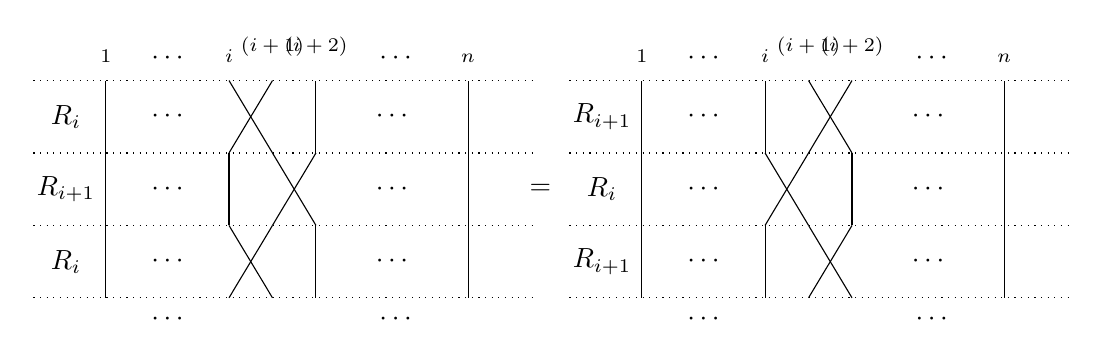
\begin{tikzpicture}[scale=0.92, baseline=(current bounding box.center)]
  % ===== 左图 =====
  \foreach \y in {0,1,2,3} {\draw[dotted] (-1.0,\y) -- (5.9,\y);}
  \draw (0,0) -- (0,3);
  \draw (5.0,0) -- (5.0,3);
  \foreach \yb/\xa/\xb/\xc in {2/1.7/2.3/2.9, 1/2.3/2.9/1.7, 0/1.7/2.3/2.9}{
    \draw (\xa,\yb+1) .. controls (\xa+0.13,\yb+0.78) and (\xb-0.13,\yb+0.22) .. (\xb,\yb);
    \draw (\xb,\yb+1) .. controls (\xb-0.13,\yb+0.78) and (\xa+0.13,\yb+0.22) .. (\xa,\yb);
    \draw (\xc,\yb) -- (\xc,\yb+1);
  }
  \node at (-0.55,2.5) {$R_{i}$};
  \node at (-0.55,1.5) {$R_{i+1}$};
  \node at (-0.55,0.5) {$R_{i}$};
  \node[above] at (0,3.12) {\scriptsize $1$};
  \node[above] at (1.7,3.12) {\scriptsize $i$};
  \node[above] at (2.3,3.2) {\scriptsize $(i+1)$};
  \node[above] at (2.9,3.2) {\scriptsize $(i+2)$};
  \node[above] at (5.0,3.12) {\scriptsize $n$};
  \node at (0.85,3.3) {$\cdots$};
  \node at (4.0,3.3) {$\cdots$};
  \node at (0.85,-0.3) {$\cdots$};
  \node at (4.0,-0.3) {$\cdots$};
  \foreach \yb in {0,1,2}{
    \node at (0.85,\yb+0.5) {$\cdots$};
    \node at (3.95,\yb+0.5) {$\cdots$};
  }
  \node at (6.0,1.5) {$=$};
  % ===== 右图 =====
  \begin{scope}[xshift=7.4cm]
  \foreach \y in {0,1,2,3} {\draw[dotted] (-1.0,\y) -- (5.9,\y);}
  \draw (0,0) -- (0,3);
  \draw (5.0,0) -- (5.0,3);
  \foreach \yb/\xa/\xb/\xc in {2/2.3/2.9/1.7, 1/1.7/2.3/2.9, 0/2.3/2.9/1.7}{
    \draw (\xa,\yb+1) .. controls (\xa+0.13,\yb+0.78) and (\xb-0.13,\yb+0.22) .. (\xb,\yb);
    \draw (\xb,\yb+1) .. controls (\xb-0.13,\yb+0.78) and (\xa+0.13,\yb+0.22) .. (\xa,\yb);
    \draw (\xc,\yb) -- (\xc,\yb+1);
  }
  \node at (-0.55,2.5) {$R_{i+1}$};
  \node at (-0.55,1.5) {$R_{i}$};
  \node at (-0.55,0.5) {$R_{i+1}$};
  \node[above] at (0,3.12) {\scriptsize $1$};
  \node[above] at (1.7,3.12) {\scriptsize $i$};
  \node[above] at (2.3,3.2) {\scriptsize $(i+1)$};
  \node[above] at (2.9,3.2) {\scriptsize $(i+2)$};
  \node[above] at (5.0,3.12) {\scriptsize $n$};
  \node at (0.85,3.3) {$\cdots$};
  \node at (4.0,3.3) {$\cdots$};
  \node at (0.85,-0.3) {$\cdots$};
  \node at (4.0,-0.3) {$\cdots$};
  \foreach \yb in {0,1,2}{
    \node at (0.85,\yb+0.5) {$\cdots$};
    \node at (3.95,\yb+0.5) {$\cdots$};
  }
  \end{scope}
\end{tikzpicture}
\]
% [Tutor Note: 上图照 p.137 重画：横向虚线为被作用的对象系，纵向实线为 $R_{i}$ 作用后保留/置换的位置，三道横带自下而上各含一个交叉。左图三道带自上而下为 $\sigma_{i},\sigma_{i+1},\sigma_{i}$，右图为 $\sigma_{i+1},\sigma_{i},\sigma_{i+1}$（$\sigma_{i}$ 表示交换第 $i$ 与第 $i+1$ 股），正是 (a) 的两端；两图给出同一置换，即辫关系式。]

\section{Serre 函子}

本章中也讨论有限型 $K$ 上三角范畴的结构，并且不假定它具有 DG 增广。将频繁应用 4.1.2 节中的自然变换与可表性。

\subsection{Serre 函子}

对 $K$ 上的三角范畴 $\cT$ 与其对象 $X$，$\Hom_{\cT}(X,\ )$、$\Hom_{\cT}(\ ,X)$ 分别定义了从 $\cT$ 到 $\mathrm{vect}(K)$ 的共变、反变上同调函子。因此，通过取 $K$-向量空间的对偶
\[
  \Hom_{\cT}(X,Y)^{*} := \Hom_{K}\bigl(\Hom_{\cT}(X,Y), K\bigr),
\]
$\Hom_{\cT}(X,\ )^{*}$、$\Hom_{\cT}(\ ,X)^{*}$ 分别成为从 $\cT$ 到 $\mathrm{vect}(K)$ 的反变、共变上同调函子。

\begin{definition}{5.71} ([9], cf.\ [10]) 设 $K$ 上的三角范畴 $\cT$ 中，存在自等价函子 $\nu \colon \cT \to \cT$，且对任意对象 $X,Y \in \cT$ 存在同型
\[
  \varphi_{X,Y} \colon \Hom_{\cT}(X,Y) \xrightarrow{\ \sim\ } \Hom_{\cT}(Y,\nu(X))^{*},
\]
并且它诱导共变、反变函子的自然等价
\begin{equation}
  \varphi_{X,*} \colon \Hom_{\cT}(X,\ ) \overset{\mathrm{n.e.}}{\simeq} \Hom_{\cT}(\ ,\nu(X))^{*}, \tag{5.35}
\end{equation}
\begin{equation}
  \varphi_{*,Y} \colon \Hom_{\cT}(\ ,Y) \overset{\mathrm{n.e.}}{\simeq} \Hom_{\cT}(Y,\nu(\ ))^{*}. \tag{5.36}
\end{equation}
此时称 $\nu$ 为 Serre 函子（Serre functor）。\end{definition}

由这个定义可得以下事实。

(5.35) 意味着函子 $\Hom_{\cT}(\ ,\nu(X))^{*}$ 由 $X$ 所表出（定义 4.17）。由补題 4.18，自然等价 $\varphi_{X,*}$ 由 $\varphi_{X,X}(\id_{X}) \in \Hom_{\cT}(X,\nu(X))^{*}$ 决定。把它表为
\begin{equation}
  \int_{X} := \varphi_{X,X}(\id_{X}) \tag{5.37}
\end{equation}
利用这个映射 $\int_{X} \colon \Hom_{\cT}(X,\nu(X)) \to K$，$\varphi_{X,Y} \colon \Hom_{\cT}(X,Y) \xrightarrow{\sim} \Hom_{\cT}(Y,\nu(X))^{*}$ 由

% [原文 p.138]
\[
  f \mapsto \varphi_{X,Y}(f) = \left(\int_{X}(f\circ\ )\colon \Hom_{\cT}(Y,\nu(X)) \to K\right)
\]
决定。由于这个对应是同构，故对非平凡的 $f$，必存在 $g \in \Hom_{\cT}(Y,\nu(X))$ 使 $\int_{X}(f\circ g) \ne 0$。

同样地，(5.36) 的自然等价 $\varphi_{X,Y} \colon \Hom_{\cT}(X,Y) \xrightarrow{\sim} \Hom_{\cT}(Y,\nu(X))^{*}$ 由
\[
  \int_{Y} := \varphi_{Y,Y}(\id_{Y}) \in \Hom_{\cT}(Y,\nu(Y))^{*}
\]
通过
\[
  f \mapsto \varphi_{X,Y}(f) = \left(\int_{Y}(\ \circ\nu(f))\colon \Hom_{\cT}(Y,\nu(X)) \to K\right)
\]
决定。由这些，得到关于 $\varphi_{X,Y}(f)$ 的等式
\[
  \int_{X}(f\circ g) = \int_{Y}(g\circ\nu(f)), \qquad g \in \Hom_{\cT}(Y,\nu(X))
\]
也就是说，由 $\int_{X}$ 决定的两个自然等价，通过自等价函子 $\nu$ 如上相互关联。反复使用这一事实，就得到 $\int_{X}(f\circ g) = \int_{Y}(g\circ\nu(f)) = \int_{\nu(X)}(\nu(f)\circ\nu(g)) = \cdots$。这在图式上意味着自等价函子 $\nu \colon \cT \to \cT$ 与自然等价 $\varphi_{X,Y}$ 的相容性
\[
\begin{tikzcd}[row sep=3em, column sep=3.8em]
  \Hom_{\cT}(X,Y) \arrow[r,"\varphi_{X,Y}"] \arrow[d,"\nu"'] & \Hom_{\cT}(Y,\nu(X))^{*}\\
  \Hom_{\cT}(\nu(X),\nu(Y)) \arrow[r,"\varphi_{\nu(X),\nu(Y)}"'] & \Hom_{\cT}(\nu(Y),\nu^{2}(X))^{*} \arrow[u,"\nu"']
\end{tikzcd}
\]

% [Tutor Note: 底本 p.138 第 8 行印作 $g \in \Hom_{\cC}(Y,\nu(X))$；据作者正誤表（2014-05-20 版）p138 条订正为 $g \in \Hom_{\cT}(Y,\nu(X))$。此处 $\cC$ 与 $\cT$ 混用系排印之误：全节只在三角范畴 $\cT$ 中讨论，且 $Y,\nu(X)$ 都是 $\cT$ 的对象。]

% [Tutor Note: 记号 $\int_{X}$ 的来源：$\int_{X} \in \Hom_{\cT}(X,\nu(X))^{*}$ 本身是从 $\Hom_{\cT}(X,\nu(X))$ 到 $K$ 的线性映射，把元素 $h \in \Hom_{\cT}(X,\nu(X))$ 送到 $\int_{X}h \in K$，这是模仿「对偶配对」的写法的作者自创记号（不是积分）。可验证：由 (5.37) 与补題 4.18，$\varphi_{X,*}$ 完全由 $\int_{X}$ 决定；而恒等式 $\int_{X}(f\circ g) = \int_{Y}(g\circ\nu(f))$ 正是 (5.35) 与 (5.36) 给出的两个自然等价在 $\Hom_{\cT}(Y,\nu(X))$ 上的配对值相等。]

Serre 函子 $\nu$ 在下述意义上与平移函子 $T \colon \cT \to \cT$ 可交换。

\begin{lemma}{5.72} ([10]) 设 $\cT$ 具有 Serre 函子 $\nu \colon \cT \to \cT$。此时，对 $\cT$ 上任意自等价函子 $F \colon \cT \to \cT$，存在自然等价 $F\circ\nu \overset{\mathrm{n.e.}}{\simeq} \nu\circ F$。\end{lemma}

\begin{proof}
存在关于 $X,Y$ 的自然等价的合成
\[
\begin{gathered}
  \Hom_{\cT}(F(Y),F(\nu(X))) \xleftarrow{\ \nu\ } \Hom_{\cT}(Y,\nu(X)) \xrightarrow{\ \varphi\ } \Hom_{\cT}(X,Y)^{*}\\
  \xleftarrow{\ \nu^{*}\ } \Hom_{\cT}(F(X),F(Y))^{*} \xleftarrow{\ \varphi^{*}\ } \Hom_{\cT}(F(Y),\nu(F(X))).
\end{gathered}
\]
利用它，构成反变函子 $\Hom_{\cT}(\ ,F(\nu(X)))$、$\Hom_{\cT}(\ ,\nu(F(X)))$ 之间的自然等价。由于 $F$ 是范畴等价函子，对任意对象 $Y' \in \cT$ 存在 $Y \in \cT$ 使 $Y' \simeq F(Y)$。利用这个同型，得到自然等价
\[
\begin{tikzcd}[row sep=2.2em, column sep=3.4em]
  \Hom_{\cT}(\ ,F(\nu(X))) \arrow[rr,"\theta"] & & \Hom_{\cT}(\ ,\nu(F(X))) \arrow[ll,"\eta"']
\end{tikzcd}
\]
由补題 4.18，上面的自然等价 $\theta,\eta$ 分别由元 $t := \theta(\id_{F\nu(X)}) \in \Hom_{\cT}(\Hom_{\cT}(F\nu(X),\nu F(X)))$、$s := \theta(\id_{\nu F(X)}) \in \Hom_{\cT}(\Hom_{\cT}(\nu F(X),F\nu(X)))$ 决定，并满足 $s\circ t = \id_{F\nu(X)}$、$t\circ s = \id_{\nu F(X)}$。由此得到自然等价

% [原文 p.139]
\[
\begin{tikzcd}[row sep=2.4em, column sep=3.6em]
  F(\nu(X)) \arrow[r, bend left=18, "t"] & \nu(F(X)) \arrow[l, bend left=18, "s"']
\end{tikzcd}
\]
从而证明完结。
\end{proof}

% [Tutor Note: 底本 p.138 末行两处印作 $t := \theta(\id_{F\nu(X)}) \in \Hom_{\cT}(\Hom_{\cT}(F\nu(X),\nu F(X)))$、$s := \theta(\id_{\nu F(X)}) \in \Hom_{\cT}(\Hom_{\cT}(\nu F(X),F\nu(X)))$，按前后文（补題 4.18 说的是 $\Hom_{\cT}(\ ,\nu(X))$ 类函子的自然变换由某个 $\Hom$ 中的元决定）应读作 $t \in \Hom_{\cT}(F\nu(X),\nu F(X))$、$s \in \Hom_{\cT}(\nu F(X),F\nu(X))$，即外层 $\Hom_{\cT}(\ )$ 是排版多出的括号。正誤表未收，照译并标注。]

其次，考虑应如何证明某个三角范畴 $\cT$ 具有 Serre 函子。首先，若 Serre 函子 $\nu$ 存在，则它是自等价函子，故存在函子 $\mu \colon S \to S$ 使 $\mu\circ\nu \overset{\mathrm{n.e.}}{\simeq} \id_{\cT} \overset{\mathrm{n.e.}}{\simeq} \nu\circ\mu$。此时，注意到自然等价 $\Hom_{\cT}(X',\nu(\ )) \overset{\mathrm{n.e.}}{\simeq} \Hom_{\cT}(\mu(X'),\mu(\nu(\ ))) \overset{\mathrm{n.e.}}{\simeq} \Hom_{\cT}(\mu(X'),\ )$ 存在，则自然等价 (5.35)、(5.36) 之存在，与它们的对偶
\begin{equation}
  \varphi^{*}_{X,*} \colon \Hom_{\cT}(X,\ )^{*} \xleftarrow{\ \sim\ } \Hom_{\cT}(\ ,\nu(X)), \tag{5.38}
\end{equation}
\begin{equation}
  \varphi^{*}_{*,X'} \colon \Hom_{\cT}(\ ,X')^{*} \simeq \Hom_{\cT}(\mu(X'),\ ) \tag{5.39}
\end{equation}
之存在等价。这些意味着 $\Hom_{\cT}(X,\ )^{*}$、$\Hom_{\cT}(X',\ )^{*}$ 分别由 $\nu(X)$、$\mu(X')$ 所表出。

% [Tutor Note: 底本 p.139 印作「関手 $\mu \colon S \to S$」，按上下文（自等价函子 $\nu \colon \cT \to \cT$ 的逆）应为 $\mu \colon \cT \to \cT$；正誤表未收，照印本翻译并标注。]

\begin{lemma}{5.73} ([9]) 对 $K$ 上有限型三角范畴 $\cT$，以下等价：
\begin{itemize}
  \item[(i)] $\cT$ 具有 Serre 函子。
  \item[(ii)] 对所有 $X,X' \in \cT$，$\Hom_{\cT}(X,\ )^{*}$、$\Hom_{\cT}(\ ,X')^{*}$ 都可表。
\end{itemize}
\end{lemma}

\begin{proof}
由于 (i)$\Rightarrow$(ii) 已证，故只需证明 (ii)$\Rightarrow$(i)。把表出 $\Hom_{\cT}(X,\ )^{*}$、$\Hom_{\cT}(\ ,X')^{*}$ 的对象分别记作 $\nu(X)$、$\mu(X')$。首先证明这些对应 $X \mapsto \nu(X)$、$X' \mapsto \mu(X')$ 定义函子。对每个态射 $f \colon X \to Y$，要构成态射 $\nu(f) \colon \nu(X) \to \nu(Y)$。由态射 $f \colon X \to Y$ 所定义的自然变换
\[
  \theta(f) \colon \Hom_{\cT}(X,\ )^{*} \to \Hom_{\cT}(Y,\ )^{*}
\]
与自然等价
\[
\begin{tikzcd}[row sep=1.6em, column sep=4.4em]
  \Hom_{\cT}(\ ,\nu(X)) \arrow[r, bend left=20, "\rho(X)"] & \Hom_{\cT}(X,\ )^{*} \arrow[l, bend left=20, "\sigma(X)"']
\end{tikzcd}
\]
作合成，就构成自然变换
\[
  \theta = \sigma(Y)\circ\theta(f)\circ\rho(X) \colon \Hom_{\cT}(\ ,\nu(X)) \to \Hom_{\cT}(\ ,\nu(Y)),
\]
于是态射 $\nu(f) := \theta_{\nu(X)}(\id_{\nu(X)})$ 得以定义（cf.\ 补題 4.18）。由这一构成可知 $\nu \colon \cT \to \cT$ 是函子。同样地可证 $\mu \colon \cT \to \cT$ 也是函子。进而，由今所构成的自然等价的合成
\[
  \Hom_{\cT}(X,\ ) \xrightarrow{\ \sim\ } \Hom_{\cT}(\ ,\nu(X))^{*} \xleftarrow{\ \sim\ } \Hom_{\cT}(\mu(\nu(X)),\ ),
\]
\[
  \Hom_{\cT}(\ ,X') \xrightarrow{\ \sim\ } \Hom_{\cT}(\mu(X'),\ )^{*} \xleftarrow{\ \sim\ } \Hom_{\cT}(\ ,\nu(\mu(X)))
\]
得到自然等价 $\mu\circ\nu \overset{\mathrm{n.e.}}{\simeq} \id_{\cT} \overset{\mathrm{n.e.}}{\simeq} \nu\circ\mu$。
\end{proof}

% [Tutor Note: 底本 p.139 此处第二行末印作 $\Hom_{\cT}(\ ,\nu(\mu(X)))$，按对称性（同第一行的 $\mu(\nu(X))$）应为 $\nu(\mu(X'))$；正誤表未收，照印本翻译并标注。另：底本「(i)⇒(ii) は既に示したので」之后所印箭头方向为 (ii)⇐(i)，就文意只能是 (ii)⇒(i)，此处按文意译。]

% [原文 p.140]
由这个证明可以看出，Serre 函子若存在，则除自然等价外唯一（cf.\ [10, 命题 1.5]）。事实上，它进而构成三角函子 [9]。

% [Tutor Note: 「さらに三角関手を成す」是 [9]（Bondal–Kapranov）中的结果，即 Serre 函子 $\nu$ 自动是正合三角函子（与平移 $T$ 交换，见补題 5.72，故 $T\circ\nu \simeq \nu\circ T$；并把正合三角序列送到正合三角序列）。这一点在定理 5.74(b) 的计算 $\nu(E_{i}) \simeq T^{n-1}L^{n-1}(E_{i})$ 中用到。]

对某个 $n = 1,2,\ldots$，也存在 $\nu \simeq T^{n}$ 的 Serre 函子的三角范畴。这样的三角范畴由对应的几何学取名，称为 Calabi–Yau 范畴（Calabi–Yau category）。这样的三角范畴 $\cT$，由于对所有对象 $X \in \cT$ 都有 $0 \ne \Hom_{\cT}(X,X)^{*} \simeq \Hom_{\cT}(X,\nu(X)) = \Hom_{\cT}(X,T^{n}(X))$，故不具有例外对象。这样一来，具有例外生成系的三角范畴在某种程度上是特别的东西，但它们包含足够重要的三角范畴类。在 6.5 节中讨论这样的三角范畴。

% [Tutor Note: 「$0 \ne \Hom_{\cT}(X,X)^{*}$」对 $X \ne 0$ 成立是因为 $\id_{X} \ne 0$（在 $K$ 上三角范畴中 $X \ne 0$ 时 $\id_{X}$ 非零），故其对偶 $\Hom_{\cT}(X,X)^{*}$ 非零，于是 $\Hom_{\cT}(X,\nu(X)) \ne 0$；但例外对象 $E$ 要求 $\Hom_{\cT}(E,T^{k}(E)) = 0$（$k \ne 0$），若 $\nu \simeq T^{n}$（$n \ge 1$）则 $k = n \ne 0$ 处非零，矛盾。故 Calabi–Yau 范畴没有例外对象，也就不可能有例外生成系。这是本书 5.6 节与 5.7 节的分水岭。]

\subsection{例外对象系与 Serre 函子}

\begin{theorem}{5.74} 设 $(E_{1},\ldots,E_{n})$ 为 $K$ 上有限型三角范畴 $\cT$ 的例外生成系。此时，
\begin{itemize}
  \item[(a)] $\cT$ 具有 Serre 函子 $\nu \colon \cT \to \cT$；
  \item[(b)] 对每个 $i = 1,\ldots,n$，$\nu(E_{i}) \simeq T^{n-1}L^{n-1}(E_{i})$。
\end{itemize}
（(a) 是 [9]，(b) 是 [7]。）\end{theorem}

以下本节中说明定理 5.74(a)、(b) 的证明概要。首先为此准备语言。

\begin{definition}{5.75} 设给定了加法范畴 $\mathcal{A}$ 的全子范畴 $\mathcal{B}$。对任意对象 $B \in \mathcal{B}$，由满足 $\Hom_{\cT}(B,C) = 0$ 的对象 $C \in \cT$ 组成的 $\mathcal{A}$ 的全子范畴记作 $\mathcal{B}^{\perp}$，并称为 $\mathcal{T}$ 中 $\mathcal{B}$ 的右正交全子范畴（right orthogonal）。同样地可定义 $\mathcal{B}$ 的左正交全子范畴（left orthogonal）${}^{\perp}\mathcal{B}$。当 $\mathcal{A}$ 是三角范畴、$\mathcal{B}$ 是其全三角子范畴时，注意 $\mathcal{B}^{\perp}$、${}^{\perp}\mathcal{B}$ 都是全三角子范畴。\end{definition}

% [Tutor Note: 底本 p.140 定義 5.75 中印作「$\Hom_{\cT}(B,C) = 0$ となる対象 $C \in \cT$」，就定义（$\mathcal{B} \subset \mathcal{A}$，$\mathcal{B}^{\perp}$ 是 $\mathcal{A}$ 的全子范畴）应为 $\Hom_{\mathcal{A}}(B,C) = 0$ 与 $C \in \mathcal{A}$；正誤表未收，照印本翻译并标注。]

\begin{definition}{5.76} 称 $K$ 上有限型三角范畴 $\mathcal{A}$ 的全子范畴 $\mathcal{B}$ 具有右容许性（right admissible），是指对任意对象 $X \in \mathcal{A}$，存在 $\mathcal{A}$ 的正合三角序列
\[
  B \to A \to C \to T(B)
\]
且 $B \in \mathcal{B}$、$C \in \mathcal{B}^{\perp}$。此时称 $\mathcal{B}$ 为 $\mathcal{A}$ 的右容许全子范畴（right admissible subcategory）。

同样地，由正合三角序列
\[
  C' \to A \to B \to T(C'), \qquad C' \in {}^{\perp}\mathcal{B},\ B \in \mathcal{B}
\]
定义 $\mathcal{B}$ 的左容许性。\end{definition}

当给定 $K$ 上有限型三角范畴 $\mathcal{A}$ 的例外对象系 $\mathcal{E} = (E_{1},\ldots,E_{k})$ 时，与 $\mathcal{E}$ 的变异同样地，对任意 $A \in \mathcal{A}$，由正合三角序列
\[
  L(A) \to \RHom_{\mathcal{A}}(E_{k},A)\otimes E_{k} \to A \to TL(A)
\]

% [原文 p.141]
定义 $L(A) \in \mathcal{A}$，并反复进行，从而归纳地定义 $L^{k}(A)$：
\[
  L^{i+1}(A) \to \RHom_{\mathcal{A}}(E_{k-i},L^{i}(A))\otimes E_{k-i} \to L^{i}(A) \to TL^{i+1}(A).
\]
（把 $A$ 置于 $(E_{1},\ldots,E_{k})$ 的右侧，一个一个地向左移动，直到移动到 $E_{1}$ 的左侧。）此时，若 $j > k-i$ 则 $\Hom_{\mathcal{A}}(T^{m}E_{j},L^{i}(A)) = 0$ 成立（$m \in \Z$）。特别地，对每个 $i = 1,\ldots,k$ 有 $\Hom_{\mathcal{A}}(T^{m}E_{i},L^{k}(A)) = 0$，由这一事实可得
\[
  \langle L^{k}(A)\rangle \subset \mathcal{B}^{\perp}, \qquad \mathcal{B} = \langle E_{1},\ldots,E_{k}\rangle.
\]

\begin{lemma}{5.77} $K$ 上有限型三角范畴 $\mathcal{A}$ 的例外对象系 $(E_{1},\ldots,E_{k})$ 所生成的全三角子范畴 $\mathcal{B}$ 具有右容许性。特别地，对对象 $A \in \mathcal{A}$，存在正合三角序列
\begin{equation}
  B \to A \to T^{k}L^{k}(A) \to T(B), \qquad B \in \mathcal{B} \tag{5.40}
\end{equation}
\end{lemma}

\begin{proof}
用归纳法证明。当 $k = 0$ 时命题显然成立。现设对 $\mathcal{B} := \langle E_{1},\ldots,E_{k}\rangle$ 正合三角序列 (5.40) 存在。进而，当存在 $E_{0} \in \mathcal{A}$ 使 $(E_{0},E_{1},\ldots,E_{k})$ 成为例外对象系时，由
\[
  L^{k+1}(A) \to \RHom_{\mathcal{A}}(E_{0},L^{k}(A))\otimes E_{0} \to L^{k}(A)
\]
定义 $L^{k+1}(A)$。由八面体公理，
\[
\begin{tikzcd}[row sep=3.4em, column sep=3.6em]
  & (E_{0})^{\oplus\bullet} \arrow[d] \arrow[r, Rightarrow] & (E_{0})^{\oplus\bullet} \arrow[d] & \\
  A \arrow[r] \arrow[d, Rightarrow] & T^{k}L^{k}(A) \arrow[r] \arrow[d] & T(B) \arrow[r] \arrow[d,"T(h)"] & T(A) \arrow[d, Rightarrow]\\
  A \arrow[r] \arrow[d] & T^{k+1}L^{k+1}(A) \arrow[r] \arrow[d] & T(B') \arrow[r] \arrow[d] & T(A)\\
  {} & T((E_{0})^{\oplus\bullet}) \arrow[r, Rightarrow] & T((E_{0})^{\oplus\bullet}) & {}
\end{tikzcd}
\]
（$(E_{0})^{\oplus\bullet} := \RHom_{\mathcal{A}}(E_{0},L^{k}(A))\otimes T^{k}(E_{0})$）存在使其可交换的 $B' \in \mathcal{A}$ 与态射 $h \colon B \to B'$；而由 $(E_{0})^{\oplus\bullet}, B \in \langle E_{0},E_{1},\ldots,E_{k}\rangle =: \mathcal{B}'$ 得 $B' \in \mathcal{B}'$。因此，得到上述八面体公理中第 3 行的正合三角序列，归纳法完成。
\end{proof}

% [Tutor Note: 上图照 p.141 重画。横置的两条 $\Rightarrow$ 表示原图中两端出现的「相等」双线（同一对象）。三个方块中，左侧与右侧的竖线为 $\Rightarrow$（恒等），中间列与右侧列的竖线为八面体公理中的态射；$T(h)$ 即 $h$ 经平移所得。这一步是定理 5.74(a) 证明的关键：由 $\mathcal{B}$ 的右容许性归纳地给出 $\langle E_{0},E_{1},\ldots,E_{k}\rangle$ 的右容许性，从而（补題 5.73）$\cT$ 具有 Serre 函子。]

关于 $\mathcal{B}$ 的左容许性也成立同样的定理。

其次，讨论三角范畴 $\cT$ 的上同调函子。

\begin{definition}{5.78} 称 $K$ 上有限型三角范畴 $\mathcal{A}$ 具有右饱和性（right saturated），是指 $\mathcal{A}$ 的所有反变上同调函子都可表。$\mathcal{A}$ 具有左

% [原文 p.142]
（承前页）饱和性（right saturated）是指 $\mathcal{A}$ 的所有共变上同调函子都可表。兼有右饱和性、左饱和性两者时，称其具有饱和性。\end{definition}

% [Tutor Note: 底本 p.141 末与 p.142 首把「左飽和性」的英文也印作 (right saturated)；按定义（反变/共变上同调函子分别可表）左饱和性应为 left saturated。正誤表未收，照印本翻译并标注。]

\begin{example}{5.79} 对 $K$ 上有限型三角范畴 $\mathcal{A}$ 的例外对象 $E \in \mathcal{A}$，$\langle E\rangle$ 具有饱和性。\end{example}

% [Tutor Note: 例 5.79 的依据：$\langle E\rangle$ 的对象是 $E$ 的有限次平移与映射锥的迭代，其上的 $K$-向量空间结构完全由 $\Hom_{\cT}(E,T^{k}(E))$（$k=0$ 时为 $K$、$k \ne 0$ 时为 $0$）决定，故任一反变/共变上同调函子在 $\langle E\rangle$ 上只依赖一个有限维 $K$-向量空间，必可表。这是 5.7.2 节归纳（定理 5.74(a) 的证明）的初始情形 $k=0$。]

\begin{lemma}{5.80} ([9]) 设给定 $K$ 上有限型三角范畴 $\mathcal{A}$ 的具有右容许性的全三角子范畴 $\mathcal{B}$。若 $\mathcal{B}, \mathcal{B}^{\perp}$ 具有右饱和性，则 $\mathcal{A}$ 也具有右饱和性。若 $\mathcal{B}, \mathcal{B}^{\perp}$ 具有左饱和性，则 $\mathcal{A}$ 也具有左饱和性。\end{lemma}

\begin{proof}
就右饱和性的情形叙述。对某个反变上同调函子 $F \colon \mathcal{A} \to \mathrm{vect}(K)$，由 $\mathcal{B}, \mathcal{B}^{\perp}$ 的右饱和性，存在 $B_{0} \in \mathcal{B},\ C_{0} \in \mathcal{B}^{\perp}$ 使
\[
  F|_{\mathcal{B}} \overset{\mathrm{n.e.}}{\simeq} \Hom_{\mathcal{B}}(\ ,B_{0}), \qquad
  F|_{\mathcal{B}^{\perp}} \overset{\mathrm{n.e.}}{\simeq} \Hom_{\mathcal{B}^{\perp}}(\ ,C_{0}).
\]
进而，也存在表出反变函子 $\Hom_{\mathcal{B}^{\perp}}(\ ,B_{0})$ 的对象 $C_{1} \in \mathcal{B}^{\perp}$。对相应的自然等价 $\theta \colon \Hom_{\mathcal{B}^{\perp}}(\ ,C_{1}) \to \Hom_{\mathcal{B}^{\perp}}(\ ,B_{0})$，置 $\gamma := \theta(\id_{C_{1}}) \in \Hom_{\mathcal{B}^{\perp}}(C_{1},B_{0})$（cf.\ 补題 4.18）。进而，把 $F(\gamma) \colon F(B_{0}) \to F(C_{1})$ 下 $\id_{B_{0}}$ 的像置为 $\varphi := F(\gamma)(\id_{B_{0}})$。利用这些，$C_{2} \in \mathcal{B}^{\perp}$ 以及 $X \in \mathcal{A}$ 由可换图式与 2 个正合三角序列
\begin{equation}
\begin{tikzcd}[row sep=2.6em, column sep=2.8em]
  T^{-1}(C_{2}) \arrow[r] \arrow[d, Rightarrow] & C_{1} \arrow[r,"\varphi"] \arrow[d,"\gamma"] & C_{0} \arrow[r] & C_{2}\\
  T^{-1}(C_{2}) \arrow[r] & B_{0} \arrow[r] & X \arrow[r] & C_{2}
\end{tikzcd}
\tag{5.41}
\end{equation}
定义。

其次证明 $X$ 表出 $F$。在 $\mathcal{B}, \mathcal{B}^{\perp}$ 上 $F$ 与 $\Hom_{\mathcal{A}}(\ ,X)$ 自然同值是容易看出的。另一方面，对 (5.41) 中的正合三角序列 $B_{0} \to X \to C_{2}$ 应用 $F$ 或 $\Hom_{\mathcal{A}}(\ ,X)$ 所得的长正合列是 $\mathrm{vect}(K)$ 中的，而由于 $F(B_{0}) \simeq \Hom_{\mathcal{A}}(B_{0},X)$、$F(C_{2}) \simeq \Hom_{\mathcal{A}}(C_{2},X)$，可以构成同型
\[
  F(X) \simeq \Hom_{\mathcal{A}}(X,X).
\]
由补題 4.18，通过这个同型，对应于 $\id_{X}$ 的 $F(X)$ 的元定义了自然变换
\[
  \eta \colon \Hom_{\mathcal{A}}(\ ,X) \to F,
\]
且 $\eta$ 在 $\mathcal{B}, \mathcal{B}^{\perp}$ 上是自然等价。要证明 $\eta$ 在 $\mathcal{A}$ 中是自然等价，即对任意对象 $Y \in \mathcal{A}$ 证明 $\eta_{Y} \colon \Hom_{\mathcal{A}}(Y,X) \to F(Y)$ 是同型。由于 $\mathcal{B}$ 具有右容许性，存在正合三角序列
\[
  B \to Y \to C, \qquad B \in \mathcal{B},\ C \in \mathcal{B}^{\perp}
\]

% [原文 p.143]
故由 $\eta_{B}, \eta_{C}$ 是同型以及五项引理（补題 4.53；cf.\ 补題 5.12），可得 $\eta_{Y}$ 是同型。
\end{proof}

由这个补題，定理 5.74(a) 可得。设 $\cT$ 具有例外生成系 $(E_{1},\ldots,E_{n})$。各 $\mathcal{B}_{i} := \langle E_{i}\rangle$ 具有饱和性。在 $\langle E_{n-1},E_{n}\rangle$ 中 $\mathcal{B}_{n}^{\perp} = \mathcal{B}_{n-1}$，且 $\mathcal{B}_{n}$ 具有右容许性，故 $\langle E_{n-1},E_{n}\rangle$ 具有饱和性。反复进行这一操作，可知 $\cT$ 具有饱和性；也就是说，由补題 5.73，$\cT$ 具有 Serre 函子。\hfill$\square$

% [Tutor Note: 这里用到「$\mathcal{B}_{n}^{\perp} = \mathcal{B}_{n-1}$」：在 $\mathcal{A}_{n} := \langle E_{n-1},E_{n}\rangle$ 中，$\langle E_{n}\rangle^{\perp} = \langle E_{n-1}\rangle$（由补題 5.66 型计算：与 $E_{n}$ 正交的例外对象必与 $E_{n-1}$ 同构、与其平移等价）。再由补題 5.80（取 $\mathcal{B} = \mathcal{B}_{n}$ 右容许）知 $\mathcal{A}_{n}$ 饱和，然后对 $\langle E_{n-2},E_{n-1},E_{n}\rangle$ 重复，共 $n$ 步得到 $\langle E_{1},\ldots,E_{n}\rangle = \cT$ 饱和。]

\begin{proof}[\bfseries 定理 5.74(b) 的证明]
对三角范畴 $\cT$ 的例外生成系 $\langle E_{1},\ldots,E_{n}\rangle$，只需证明反变函子 $\Hom_{\cT}(E_{n},\ )^{*}$ 由 $\nu(E_{n}) := T^{n-1}L^{n-1}(E_{n})$ 表出。对任意对象 $X \in \cT$，由 $\mathcal{B} := \langle E_{1},\ldots,E_{n-1}\rangle$ 的右容许性（补題 5.77），存在正合三角序列
\[
  B \to X \to T^{n-1}L^{n-1}(X), \qquad B \in \mathcal{B}.
\]
对其应用上同调函子 $\Hom_{\cT}(E_{n},\ )$，得到同型
\[
  \Hom_{\cT}(E_{n},X) \simeq \Hom_{\cT}(E_{n},T^{n-1}L^{n-1}(X))
\]
（注意 $E_{n} \in {}^{\perp}\mathcal{B}$）。同样地，应用反变上同调函子 $\Hom_{\cT}(\ ,\nu(E_{n}))$，得到同型
\[
  \Hom_{\cT}(X,\nu(E_{n})) \simeq \Hom_{\cT}(T^{n-1}L^{n-1}(X),\nu(E_{n})).
\]
由于 $T^{n-1}L^{n-1}(X) \in \langle\nu(E_{n})\rangle = \mathcal{B}^{\perp}$，$T^{n-1}L^{n-1}(X)$ 与 $\nu(E_{n})$ 的平移 $\nu(E_{n})[*]$ 们的直和同型。因此
\[
  \Hom_{\cT}(E_{n},T^{n-1}L^{n-1}(X))^{*} \xleftarrow{\ \sim\ } \Hom_{\cT}(T^{n-1}L^{n-1}(X),\nu(E_{n}))
\]
成立。把这些合起来，就得到点线部分的自然等价
\[
\begin{tikzcd}[row sep=3.6em, column sep=4.2em]
  \Hom_{\cT}(E_{n},T^{n-1}L^{n-1}(X))^{*} & \Hom_{\cT}(T^{n-1}L^{n-1}(X),\nu(E_{n})) \arrow[l,"\sim" above]\\
  \Hom_{\cT}(E_{n},X)^{*} \arrow[u,"\sim" left] & \Hom_{\cT}(X,\nu(E_{n})) \arrow[l,dashed,"\sim" above] \arrow[u,"\sim" right]
\end{tikzcd}
\]
\end{proof}

% [Tutor Note: 图中虚线部分即所要构造的自然等价：上边一条由「$T^{n-1}L^{n-1}(X)$ 是 $\nu(E_{n})$ 的平移之直和」得到，左右两条由上面两个同型得到，底边一条为虚线的目标。取 $X = E_{n}$ 可验：$\Hom_{\cT}(E_{n},E_{n})^{*} \simeq K \simeq \Hom_{\cT}(E_{n},T^{n-1}L^{n-1}(E_{n}))^{*}$，与 $\nu(E_{n}) := T^{n-1}L^{n-1}(E_{n})$ 的定义相符。]

最后，叙述应用以上讨论对辫关系式（命题 5.69(a)）的证明。对 $K$ 上有限型三角范畴 $\cT$ 的例外对象系 $\mathcal{E} := (E_{1},\ldots,E_{n})$，关于左变异的关系式
\[
  L_{i+1}L_{i}L_{i+1}(E) = L_{i}L_{i+1}L_{i}(E), \qquad i = 2,\ldots,n-1
\]
加以说明。$L_{i+1}L_{i}L_{i+1}$、$L_{i}L_{i+1}L_{i}$ 分别只改变 $E_{i-1},E_{i},E_{i+1}$，保持其余不变。特别是，
\[
  L_{i+1}L_{i}L_{i+1}(E_{i-1},E_{i},E_{i+1}) = (L^{2}(E_{i+1}),L(E_{i}),E_{i-1}),
\]
而

% [原文 p.144]
对 $L_{i}(E_{i-1},E_{i},E_{i+1}) = (L(E_{i}),E_{i-1},E_{i+1}) =: (E'_{i-1},E'_{i},E'_{i+1})$，有
\[
\begin{aligned}
  L_{i}L_{i+1}L_{i}(E_{i-1},E_{i},E_{i+1})
  &= L_{i}L_{i+1}(E'_{i-1},E'_{i},E'_{i+1}) = (L^{2}(E'_{i+1}),E'_{i-1},E'_{i})\\
  &= (L^{2}(E'_{i+1}),L(E_{i}),E_{i-1}),
\end{aligned}
\]
故只需证明等式 $L^{2}(E_{i+1}) = L^{2}(E'_{i+1})$。

今设 $\mathcal{A} := \langle E_{i-1},E_{i},E_{i+1}\rangle \subset \cT$、$\mathcal{B} := \langle E_{i-1},E_{i}\rangle \subset \mathcal{A} \subset \cT$。注意到 $\langle E'_{i-1},E'_{i}\rangle = \mathcal{B}$，则 $L^{2}(E_{i+1}), L^{2}(E'_{i+1})$ 都是 $\mathcal{B}^{\perp}$ 的元，特别地都是 $\cT$ 的例外对象。也就是说，存在某个整数 $n \in \Z$ 使
\begin{equation}
  L^{2}(E_{i+1}) \simeq L^{2}(E'_{i+1})[n] \in \cT \tag{5.42}
\end{equation}
成立。另一方面，由 $\mathcal{A}$ 中的 Serre 函子 $\nu_{\mathcal{A}} \colon \mathcal{A} \to \mathcal{A}$，存在 $L^{2}(E_{i+1}), L^{2}(E'_{i+1})$ 之间的同型
\[
  L^{2}(E_{i+1})[2] \simeq \nu_{\mathcal{A}}(E_{i+1}) \simeq L^{2}(E'_{i+1})[2] \in \mathcal{A}.
\]
由此证明了 $L^{2}(E_{i+1}) \simeq L^{2}(E'_{i+1}) \in \cT$。\hfill$\square$

% [Tutor Note: 收尾推导的关键是「平移只能差整数次」：$L^{2}(E_{i+1}),L^{2}(E'_{i+1})$ 都是 $\mathcal{B}^{\perp}$ 中的例外对象，例外对象之间的同构类只差平移，故 (5.42) 中的 $n$ 存在。再用 $\mathcal{A}$ 的 Serre 函子把 $E_{i+1}$ 送到 $L^{2}(E_{i+1})[2]$，两边同时平移 2 次即可消去 $n$（因 $\nu_{\mathcal{A}}$ 与平移可换，补題 5.72）。这也印证了 5.7.1 节强调的「$\nu$ 与 $T$ 可换」。]

\para{文献} 关于三角范畴，有 Gelfand–Manin [17]、Kashiwara–Schapira [34]、Weibel [56]、Neeman [47] 等。关于三角 DG 范畴（5.5 节），仅举原论文 [8]。也存在 DG 范畴局部化的表述 [12]。关于例外对象系的变异（5.6 节）与 Serre 函子（5.7 节），也仅举本文所引用的原论文。作为三角范畴的具体构成，本书未叙述但重要者，有作为 Frobenius 范畴（Frobenius category）的稳定同伦范畴的三角范畴构成（Happel [18, p11]），以及其名称由来的同伦论中的\textbf{稳定同伦范畴}（stable homotopy category）（cf.\ 土屋 [55]）等。
